
% documentclass options:
% ngerman is needed for hyphenation if the thesis contains parts written in German
% BCOR is binding correction
% if you'd rather have a one sided thesis, add `onside' to the documentclass
\documentclass[11pt, a4paper, BCOR=10mm, english, ngerman]{scrbook}
% include all packages and define commands in setup.tex

%------------------------------------------------------------------------------
%       package includes
%------------------------------------------------------------------------------
    % font encoding is set up for pdflatex, for other environments see
    % http://tex.stackexchange.com/questions/44694/fontenc-vs-inputenc
    \usepackage[T1]{fontenc}  % 8-bit fonts, improves handling of hyphenations
    \usepackage[utf8x]{inputenc}
    % provides `old' commands for table of contents. Eases the ability to switch
    % between book and scrbook
    \usepackage{scrhack}
	\usepackage{helvet}
	\renewcommand{\familydefault}{\sfdefault}
    % ------------------- layout, default -------------------
    % adjust the style of float's captions, separated from text to improve readabilty
    \usepackage[labelfont=bf, labelsep=colon, format=hang, textfont=singlespacing]{caption}
    \let\counterwithout\relax
	\let\counterwithin\relax
    \usepackage{chngcntr}  % continuous numbering of figures/tables over chapters
    \counterwithout{equation}{chapter}
    \counterwithout{figure}{chapter}
    \counterwithout{table}{chapter}

    % Uncomment the following line if you switch from scrbook to book
    % and comment the setkomafont line
    %\usepackage{titlesec}  % remove "Chapter" from the chapter title
    %\titleformat{\chapter}[hang]{\bfseries\huge}{\thechapter}{2pc}{\huge}
    \setkomafont{chapter}{\normalfont\bfseries\huge}

    \usepackage{setspace}  % Line spacing
    \onehalfspacing
    % \doublespacing  % uncomment for double spacing, e.g. for annotations in correction

    % ------------------- functional, default-------------------
    \usepackage[dvipsnames]{xcolor}  % more colors
    \usepackage{array}  % custom format per column in table - needed on the title page
    \usepackage{graphicx}  % include graphics
    \usepackage{subfig}  % divide figure, e.g. 1(a), 1(b)...
    \usepackage{amsmath}  % |
    \DeclareMathOperator{\Tr}{Tr}
    \usepackage{amsthm}   % | math, bmatrix etc
    \usepackage{amsfonts} % |
    \usepackage{calc}  % calculate within LaTeX
    \usepackage{epstopdf}
    \usepackage{printlen}
    \usepackage{layouts}
	\epstopdfsetup{outdir=./}
    \usepackage[unicode=true,bookmarks=true,bookmarksnumbered=true,
                bookmarksopen=true,bookmarksopenlevel=1,breaklinks=false,
                pdfborder={0 0 0},backref=false,colorlinks=false]{hyperref}
                \usepackage[separate-uncertainty=true]{siunitx}
    \DeclareSIUnit\molar{\mole\per\cubic\deci\metre}
    \DeclareSIUnit\Molar{\textsc{m}}
    \DeclareSIUnit\gauss{G}
    \DeclareSIUnit\Molar{\textsc{m}}
    \usepackage{braket}


    %==========================================
    % You might not need the following packages, I only included them as they
    % are needed for the example floats
    % ------------------- functional, custom -------------------
    \usepackage{algorithm,algpseudocode}
    \usepackage{bm}  % bold greek variables (boldmath)
    \usepackage{tikz}
    \usetikzlibrary{positioning}  % use: above left of, etc

    % Improves general appearance of the text
    \usepackage[protrusion=true,expansion=true, kerning]{microtype}

%------------------------------------------------------------------------------
%       (re)new commands / settings
%------------------------------------------------------------------------------
    % ----------------- referencing ----------------
    \newcommand{\secref}[1]{Section~\ref{#1}}
    \newcommand{\chapref}[1]{Chapter~\ref{#1}}
    \renewcommand{\eqref}[1]{Equation~(\ref{#1})}
    \newcommand{\figref}[1]{Figure~\ref{#1}}
    \newcommand{\tabref}[1]{Table~\ref{#1}}

    % ------------------- colors -------------------
    \definecolor{darkgreen}{rgb}{0.0, 0.5, 0.0}
    % Colors of the Albert Ludwigs University as in
    % https://www.zuv.uni-freiburg.de/service/cd/cd-manual/farbwelt
    \definecolor{UniBlue}{RGB}{0, 74, 153}
    \definecolor{UniRed}{RGB}{193, 0, 42}
    \definecolor{UniGrey}{RGB}{154, 155, 156}


    % ------------------- layout -------------------
    % prevents floating objects from being placed ahead of their section
    \let\mySection\section\renewcommand{\section}{\suppressfloats[t]\mySection}
    \let\mySubSection\subsection\renewcommand{\subsection}{\suppressfloats[t]\mySubSection}


    % ------------------- marker commands -------------------
    % ToDo command
    \newcommand{\todo}[1]{\textbf{\textcolor{red}{(TODO: #1)}}}
    \newcommand{\extend}[1]{\textbf{\textcolor{darkgreen}{(EXTEND: #1)}}}
    % Lighter color to note down quick drafts
    \newcommand{\draft}[1]{\textbf{\textcolor{NavyBlue}{(DRAFT: #1)}}}


    % ------------------- math formatting commands -------------------
    % define vectors to be bold instead of using an arrow
    \renewcommand{\vec}[1]{\mathbf{#1}}
    \newcommand{\mat}[1]{\mathbf{#1}}
    % tag equation with name
    \newcommand{\eqname}[1]{\tag*{#1}}


    % ------------------- pdf settings -------------------
    % ADAPT THIS
    \hypersetup{pdftitle={Hyperpolarization in NMR and MRI using Sabre},
                pdfauthor={Philipp Rovedo},
                pdfsubject={PhD thesis at the Albert Ludwig University of Freiburg},
                pdfkeywords={hyperpolarization, sabre, NMR, MRI, 15N},
                pdfpagelayout=OneColumn, pdfnewwindow=true, pdfstartview=XYZ, plainpages=false}


    %==========================================
    % You might not need the following commands, I only included them as they
    % are needed for the example floats

    % ------------------- Tikz styles -------------------
    \tikzset{>=latex}  % arrow style


    % ------------------- algorithm ---------------------
    % Command to align comments in algorithm
    \newcommand{\alignedComment}[1]{\Comment{\parbox[t]{.35\linewidth}{#1}}}
    % define a foreach command in algorithms
    \algnewcommand\algorithmicforeach{\textbf{foreach}}
    \algdef{S}[FOR]{ForEach}[1]{\algorithmicforeach\ #1\ \algorithmicdo}

\begin{document}
    \pagestyle{empty} % no header and no page number
    % disable hyper links to remove warning "destination with same identifier"
    % this means within this section nothing can be referenced with a hyperlink
    \hypersetup{pageanchor=false}
    
    % enable/disable, depending on your chosen language
    % !TEX root = ../thesis_main.tex

\begin{titlepage}
\begin{center}

\newcommand{\HorizontalLine}{\rule{\linewidth}{0.3mm}}

{\Large PHD Thesis}\\[1.3cm]


% _____________________________________________________________________________
\HorizontalLine \\[0.4cm]
\begin{spacing}{3}
    {\huge \bfseries $^1$H and $^{15}$N hyperpolarization using SABRE} \\
\end{spacing}
\begin{spacing}{2}
    {\Large \bfseries Experimental approaches and hardware designs for continuous and batch hyperpolarization}\\
\end{spacing}
\HorizontalLine \\[1.5cm]
% _____________________________________________________________________________


	{\Huge Philipp Rovedo} \\[2cm]


\begin{tabular}[hc]{>{\huge}l >{\huge}l}
  Examiner: & Prof. Dr. J\"urgen Hennig \\[0.3cm]
  Adviser: & Prof Dr. Jan H\"ovener \\[1.2cm]
\end{tabular}
\vfill  % move the following text to the bottom

\Large {
    Albert-Ludwigs-University Freiburg\\
    Faculty of Physics\\
    Department of Radiology\\
    Chair for Medical Physics\\[1cm]

    October 05\textsuperscript{th}, 2017\\
}
\end{center}
\end{titlepage}

% title page back
\ \vfill \ \\  % at least one space required before vfill
\
\textbf{Writing period}            \smallskip{} \\
05.\,07.\,2017 -- 05.\,10.\,2017   \bigskip{} \\
\
\textbf{Examiner}                  \smallskip{} \\
Prof. Dr. J\"urgen Hennig               \bigskip{} \\
\
\textbf{Advisers}                  \smallskip{} \\
PD Dr. Jan H\"ovener

	%\include{chapters/0_0-titlepage_de}
    
    \pagestyle{plain} % remove chapter name from top, page number at the bottom
    \frontmatter  % roman page numbers
    % !TEX root = ../thesis_main.tex
% official declaration from the examination office; to be sure double
% check the wording on their website
% (https://www.tf.uni-freiburg.de/studies/exams/thesis/thesis_formatting.html#erklaerung)

\chapter*{Declaration}

I hereby declare, that I am the sole author and composer of my thesis and that no other sources or learning aids, other than those listed, have been used. Furthermore, I declare that I have acknowledged the work of others by providing detailed references of said work.  \newline
I hereby also declare, that my Thesis has not been prepared for another examination
or assignment, either wholly or excerpts thereof.
\\[3\normalbaselineskip]
\begin{tabular}{p{\textwidth/2} l}
  \rule{\textwidth/3}{0.4pt}   &   \rule{\textwidth/3}{0.4pt} \\
  Place, Date                  &   Signature
\end{tabular}

    \chapter*{Abstract}
foo bar


    \chapter{Deutsche Zusammenfassung}
Diese Arbeit besch\a ftigt sich mit hyperpolarisierung, also der 

    \tableofcontents
    \listoffigures
    \listoftables
    \listofalgorithms
    \hypersetup{pageanchor=true}  % re-enable hyperlinking

    \mainmatter  % Arabic page numbers
    \def\input@path{{/home/philipp/Documents/thesis/figures/}}
    % !TEX root = ../thesis_main.tex
\chapter{Introduction}
\label{chap:introduction}
    \section{Hyperpolarization}
    This work is all about hyperpolarization (HP), which can be described as the magnetization of spins exceeding their thermal equilibrium magnetization levels. The range of methods for reaching this goal is wide \cite{johannesson_dynamic_2009,hirsch_brute-force_2015,duhamel_xenon-129_2001,fain_imaging_2010, bowers_parahydrogen_1987-2, adams_reversible_2009-2}, this work is focused on chemically induced hyperpolarization using parahydrogen \cite{green_theory_2012-1}.
    The HP of nuclear spins promises to overcome MRI's greatest impediment, its low polarization and thus low sensitivity. In fact, $^{13}C$ HP has been used successfully in metabolic MRI where it delivered significant insights into cancer metabolism in vivo \cite{golman_cardiac_2008}. Mostly, hyperpolarized small molecules in solution are produced externally in a polarizer \cite{ardenkjaer-larsen_present_2016}, followed by transfer, administration and imaging in a conventional MR system of \SI{1.5}{\tesla} or more. From the moment of its production, HP decays with a characteristic time constant $T_1$ that depends on the magnetic field but rarely exceeds one minute. However, if the sample is exposed to a magnetic field below a critical value, then rapid relaxation will occur and the polarization lost. Furthermore, during imaging, the transverse magnetization decays according to $T_2$ which is estimated to be of the order of \SI{100}{\second} to  \SI{0.1}{\second}. Thus, over time, polarization is lost to the in vivo measurement by readout, dilution, excretion and relaxation. Despite these challenges, impressive results have been obtained with respect to medical diagnostics in both mice and man through the injection of a single bolus of hyperpolarized agent. Whilst pyruvate is receiving great attention, no other agents have yet been injected into man as the regulatory approval process is difficult to cross. Progress to bypass relaxation is however prospering with research into long-lived magnetization of single nuclei like Lithium-64\cite{van_heeswijk_hyperpolarized_2009} or Silicon-295 \cite{kwiatkowski_nanometer_2017} and long-lived quantum states of multi-atomic systems\cite{pileio_storage_2010, noauthor_y._nodate} being particularly noteworthy. Recently, a method to continuously hyperpolarize  nuclear spins by means of parahydrogen (pH2) and reversible exchange, Sabre, has emerged \cite{adams_reversible_2009-2, hovener_continuous_2014-1}. It offers the potential of repolarizing spins continuously in the presence of pH2. Its biological applicability, though, is limited because of the use of toxic methanol as the solvent as well as target molecules with limited biocompatibility. In this work it is shown that more biologically relevant agents can be hyperpolarized continuously in aqueous solution \cite{truong_irreversible_2014-1}. However, as we moved through experiments, it became clear that re-hyperpolarization in vivo would be difficult if not impossible to achieve. Therefore, the next step was to instead generate high batch magnetization instead of a lower, but renewable magnetization. This goal was aimed towards the same parahydrogen based SABRE method, and, as an additional step, the focus was shifted from $^1H$ HP to X-nuclei, particularly $^{15}N$\cite{truong_15n_2015-1}. The advantage here is that relaxation times can be longer and there is no background signal from the usually widely available water in biomedical application. This aim lead to the creation of new hardware designs to optimize polarization parameters and thus increase magnetization to the highest achievable levels.
    \section{Hardware}
    The hardware used in HP experiments is often costly and complex to use. Dynamic nuclear polarization methods, for example, need high fields, low temperatures and careful handling of the substrate after polarization to generate high polarizations\cite{ardenkjaer-larsen_present_2016, milani_magnetic_2015,}. Additionally, polarization times are long (with a few exceptions) often making long lead times necessary. The hardware in this work was designed to be easily and cheaply manufactured with ease of use and reproducibility in mind. Many aspects of hardware design are covered: 3D-CAD design of the components, fluid path and flow design for both gases and liquids, design of electronics for control of the setup and readout of sensor data as well as construction of components of the NMR and MRI setup such as coils for static magnetic field generation, radiofrequency-pulses and signal reception. Manufacturing methods mostly used after manual constructions were milling, lathing and 3D-printing. Using the equipment built in this work, high SABRE polarized samples were produced and measured in commercially available small animal MRI. If biologically relevant tracers are found, the setup can be used for generation of highly polarized batches of sample that in-vivo will portray metabolic processes.

    % !TEX root = ../thesis_main.tex
\chapter{Theory and state of the art}\label{chap:theory}
This chapter will provide a basis for understanding the principles of this work as well as the phenomena and effects exploited in the later chapters. It will cover the most important aspects, and, of course, for a more detailed description, the cited literature may be consulted. At first, the quantum mechanical approach describing nuclei and spin systems will be given followed by a more application oriented description of the effects occurring and used in NMR and MRI.
    \section{Nuclei and Spins}
        \label{sec:theory:nucleiSpins}
        The postulation of an electron spin in 1926 \cite{uhlenbeck_ersetzung_1925, goudsmit_ontdekking_1971} and later, in 1927, of a proton spin \cite{dennison_note_1927} opened up new areas of research. The discovery opened up numerous new research topics both in basic research, especially in high energy physics, but also in directions leading to applied sciences making use of the spin properties of the nuclei. Nuclear magnetic resonance (NMR, \cite{purcell_resonance_1946-1} ) and Magnetic Resonance Imaging (MRI, \cite{mansfield_medical_1977}) are two sprouts of that development and are the basis of this thesis.
        Each atom or molecule has magnetic properties to which both electrons and the nucleus, i.e. protons and neutrons, contribute. We consider the electrons' contributions to be of a static nature because of their, compared to usual acquisition times, fast movement (Born-Oppenheimer approximation, see \ref{sec:theory:chemicalShift}) and instead turn to the nucleus' magnetic properties. As we want to manipulate nuclei electromagnetically, their magnetic momentum is the relevant physical property in this case.
        The magnetic momentum $\vec M$ of a nucleus is connected to the spin $\vec S$ by the gyromagnetic ratio $\gamma$, a nucleus specific proportionality factor \cite{balanis_advanced_nodate}:
        \begin{equation}
            \vec M = \gamma \vec S
            \label{eq:gyromagneticRatio}
        \end{equation}
        The spin can be described as and mathematically seems to behave like an angular momentum, but is not generated by particle rotation - it is rather an intrinsic property of the particle. Each of the nuclei, in literature and in the following often also simply called "spin", is described by the quantum numbers according to the quantized angular moments, using quantum numbers j and m.
        The states of the single spin and thus its spin angular momentum can be described fully by the Pauli matrices $\vec{I} = \left\{ \hat{I}_x, \hat{I}_y, \hat{I}_z\right\}$\cite{pauli_zur_1988}
            \begin{align}
                \label{equ:theory:spinStates}
                \vec I^2 \ket{j,m} &= j(j+1)\ket{j,m}\\
                \hat{I}_z \ket{j,m} &= m\ket{j,m}\\
                \hat{I}_\pm \ket{j,m} &= \sqrt{j(j+1)-m(m+1)}\ket{j,m\pm1}
            \end{align}
        where $ \hat{I}_\pm = \hat{I}_x\pm i \hat{I}_y$.
        The nucleus then has m~=~(2j~+~1) energy eigenstates that are degenerated at zero magnetic field. If a magnetic field is present though, the energy levels will split with energy differences proportional to the magnetic field strength. The splitting is known as the Zeeman energy splitting.
        \subsection{Zeeman energy splitting}
            If a particle with a spin $S\neq 0$ is exposed to a magnetic field $B_0$, it experiences an energy splitting of its spin-eigenstates due to the fact that different directions of the spins in the magnetic field now have different energies. Both the gyromagnetic ratio and the magnetic field strength determine how big that energy is:
            \begin{equation}
                E_{Z} = -\gamma m B_0
            \end{equation}
            where $E_Z$ is the Zeeman energy of the eigenstate with the magnetic quantum number m.\cite{gerlach_experimentelle_1989, bloch_nuclear_1946}. The negative sign implies that a parallel orientation with the field for particle with positive $\gamma$ is energetically favorable. For example, $^1$H and $^{15}$N, the two main nuclei considered in this work with $\gamma = \SI{42.58}{\\mega\hertz\per\tesla}$ and $\SI{-4.32}{\mega\hertz\per\tesla}$ respectively, show energy splittings into two levels ($2\cdot\tfrac{1}{2}+1$), but of about a factor of 10 stronger for $^1$H due to the by that factor larger gyromagnetic ratio. Additionally, the energetically favorable alignment is different for both nuclei because $^{15}N$ has a negative gyromagnetic ratio (see figure \ref{figure:theory:zeemanSplittings}).
            \begin{figure}
                \centering
                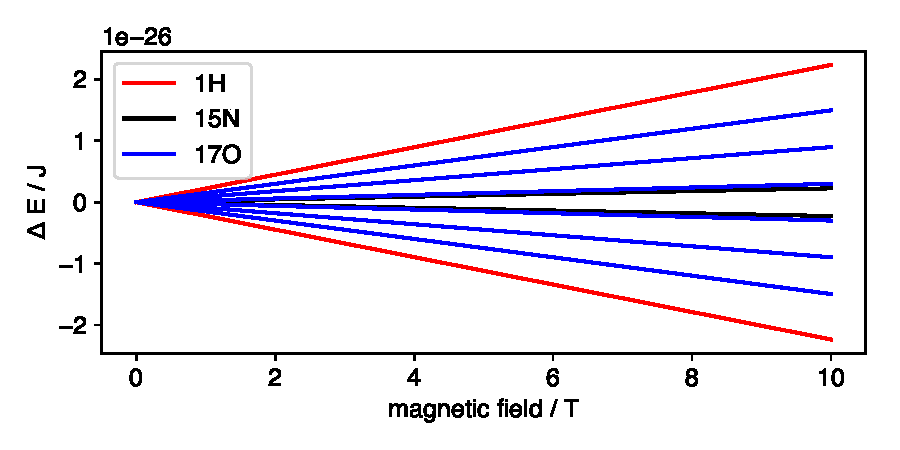
\includegraphics[width=0.9\textwidth]{/figures/theory/zeemanPlot.pdf}
                \caption[Zeeman energy splitting]{The Zeeman energy splittings of three nuclei over magnetic field. Note the difference in slopes for the spin $\tfrac{1}{2}$ nuclei $^1$H and $^{15}$N caused by the different gyromagnetic ratios. Arbitrarily, $^{17}$O, a spin $\tfrac{5}{2}$ nucleus, was plotted to visualize higher order splittings with $2 \cdot\tfrac{5}{2}+1 = 6$ energy levels. }
                \label{figure:theory:zeemanSplittings}
            \end{figure}

            When considering a spin-1/2 particle in a magnetic field along the z-axis (which is the usual choice and does not imply loss of generality), e.g. the proton as a prominent particle in NMR, its spin state can be described by the two eigenstates of $\hat{I}_z$ 
            \begin{equation}
            \ket\alpha = \begin{pmatrix}1\\0\end{pmatrix} \hspace{2 cm} \ket\beta =
            \begin{pmatrix}0\\1\end{pmatrix}
            \end{equation}
            with the eigenvalues of $\pm 1/2$. Using the Pauli matrices to construct the three angular momentum operators
            \begin{align*}
                I_x = \frac{1}{2}
                \begin{pmatrix}
                    0 & 1\\
                    1 & 0
                \end{pmatrix}, 
                I_y = \frac{1}{2}
                \begin{pmatrix}
                    0 & -i\\
                    i & 0
                \end{pmatrix}, 
                I_z = \frac{1}{2}
                \begin{pmatrix}
                    1 & 0\\
                    0 & -1
                \end{pmatrix} 
            \end{align*}
            and the corresponding shift operators $I_\pm = \frac{1}{2} \hat 1 \pm I_z$ equations \ref{equ:theory:spinStates}ff can be expressed as:
            \begin{align*}
                \vec I^2 \ket{\alpha} &= \frac{1}{2}\ket{\alpha}&\vec I^2 \ket{\beta} &= \frac{1}{2}\ket{\beta}\\
                \hat{I}_z\ket\alpha &= \frac{1}{2}\ket\alpha &\hat{I}_z\ket\beta &= -\frac{1}{2}\ket\beta\\
                \hat{I}_+\ket\alpha &= 0 &\hat{I}_+\ket\beta &= \ket\alpha\\
                \hat{I}_-\ket\alpha &= \ket\beta& \hat{I}_-\ket\beta &= 0
            \end{align*}
            Generally, every spin-1/2 particle can be in any superposition of those two eigenstates:
            \begin{equation}
                \ket\psi = c_\alpha \ket\alpha + c_\beta \ket \beta = \begin{pmatrix} c_\alpha \\
                c_\beta\end{pmatrix}
            \end{equation}
            These superposition states in general evolve under the spin Hamiltonian of the system.  To do so, usually the density matrix formalism is introduced.
             In this case, the
            expectation value of an operator for a single spin $\braket{\hat Q}$ is given by 
            \begin{equation}
            \bra\psi\hat Q\ket\psi = \left( c_\alpha^*, c_\beta^*\right)
            \begin{pmatrix}
                Q_{\alpha\alpha} Q_{\alpha\beta}\\
                Q_{\beta\alpha} Q_{\beta\beta}
            \end{pmatrix}
            \begin{pmatrix}
                c_\alpha\\
                c_\beta
            \end{pmatrix}
            \end{equation}
            as described in \cite{sakurai_modern_2017}. This is equal to the trace of the density operator
            $\ket\psi\bra\psi$ multiplied with said operator \cite{levitt_spin_nodate}
            \begin{equation}
                \braket{\hat Q} = \Tr \left\{\ket\psi\bra\psi\hat Q\right\}
            \end{equation}
            As a sample in our case does not consist of one, but many nuclei (\SI{1}{\milli\liter} of water consists of $\sim$ $7\cdot 10^{22}$ spins), the evolution of all of those spins needs to be considered to describe the system. 
            It follows that the expectation value of an observable becomes the sum of their individual statistically weighted expectation values:
            \begin{equation}
                \hat Q_{ensemble}= \bra{\psi_1}\hat Q\ket{\psi_1} + \bra{\psi_2}\hat Q\ket{\psi_2} + \hdots =
                \Tr{\left\{\left(\ket{\psi_1}\bra{\psi_1} + \ket{\psi_2}\bra{\psi_2}+ \hdots \right) \hat Q\right\}}
            \end{equation}
            The first part of the trace's argument is closely related to the density matrix which corresponds to the average sum of the individual density operators:
            \begin{equation}
                \hat\rho = \overline{\ket\psi\bra\psi} = \frac{1}{N} (\ket{\psi_1}\bra{\psi_1} + \ket{\psi_2}\bra{\psi_2} + \dots).
            \end{equation}
            For a large number of spins, the macroscopically observable value Q is then
            \begin{equation}
                Q_{macro} = \left< Q \right> = N \Tr \left( \hat{\rho} \hat{Q}\right)
            \end{equation}
            For a spin-1/2 ensemble, the density matrix in thermal equilibrium is
            \begin{equation}
                \hat \rho = \begin{pmatrix} \frac{1}{2}+\frac{1}{4}\mathbb{B}& 0\\ 0&
                \frac{1}{2}-\frac{1}{4}\mathbb{B}\end{pmatrix} = \frac {1}{2} \hat1 + \frac{1}{2} \mathbb{B}
                \hat I_z
            \end{equation}
            with $\mathbb{B} = \frac{\hbar\gamma B_0}{k_b T}$. That means that in thermal equilibrium, the non-diagonal elements (so-called coherences) are zero, while there is a slight overpopulation (see section \ref{sec:theory:HP}) of one of the two states at non vanishing magnetic fields. Through deflection from that equilibrium, coherences are populated as described in the following section.
        \subsection{Radiofrequency pulses}
        \label{sec:theory:RFPulses}
            Using the density matrix formalism, the effect of radiofrequency pulses is described by rotational operators that can be
            applied to the whole ensemble. A pulse $\hat R_\phi(\beta)$ of phase $\phi$ (corresponding
            to the axis around which magnetization is rotated) and angle $\beta$ where
            $\beta=\omega_{nut} \cdot \tau_p$ acting on a state $\ket\psi$ is described by 
            \begin{equation}
                \ket{\psi_\tau}= \hat R_\phi(\beta)\ket\psi
            \end{equation}
            Calculating the density matrix now leads to
            \begin{equation}
                \hat {\rho_\tau} = \overline{\ket{\psi_\tau}\bra{\psi_\tau}} = \overline{\hat
                    R_{\phi}(\beta)\ket\psi\bra\psi \hat R_\phi(-\beta)}
            \end{equation}
            where the overbar describes the averaging over all spins in the ensemble \cite{popov_modern_1990, chizhik_magnetic_2014} Finally, as we are considering the rotation to be the same for every single spin in the ensemble, the formula can be reduced to
            \begin{equation}
                \hat\rho_\tau = \hat R_\phi(\beta) \hat \rho \hat R_\phi(-\beta)
            \end{equation}
            where $\rho$ is the average density matrix of the ensemble meaning a rotation of the magnetization corresponds to a rotation of the density matrix. If, e.g., we consider a $\SI{90}{\degree}$ pulse around the x-axis on the previously described equilibrium for a spin-1/2 ensemble it follows \cite{hosur_scaling_1990, levitt_spin_nodate}:
            \begin{equation}
                \begin{split}
                    \hat\rho_\tau = \hat R_x(\pi/2)\hat\rho\hat R_x(-\pi/2) &= \frac{1}{2} \hat 1 +
                    \frac{1}{2} \mathbb{B}\hat R_x(\pi/2) \hat I_z \hat R_x(-\pi/2)\\
                    &=
                    \begin{pmatrix}
                        \frac{1}{2} & -\frac{1}{4i}\mathbb{B}\\
                        \frac{1}{4i}\mathbb{B}\ & \frac{1}{2}
                    \end{pmatrix}
                \end{split}
            \end{equation}
            It can be equally shown that a $\SI{180}{\degree}$ pulse inverts the populations of the diagonal elements while the coherences are untouched.  If the system is not in thermal equilibrium, the density matrix will evolve and generally relax back to its equilibrium state. If one neglects said relaxation at first, the free evolution can be described by
            \begin{equation}
                \begin{split}
                    \ket\psi_\upsilon &= \hat R_z(\Omega^0\upsilon)\ket\psi_\tau ~ \mathrm{and} \\
                    \hat\rho_\upsilon &= \hat R_z(\Omega^0\upsilon)\hat\rho_\tau\hat R_z(-\Omega^0\upsilon)
                \end{split}
            \end{equation}
            where $\upsilon$ is the free evolution time and $\Omega_0$ is the frequency offset off the central, rotating frame frequency. Only a time dependent phase $\exp{(\Omega^0 \upsilon)}$ is added to the coherences that way and the populations stay constant. This confirms the macroscopic observation that the ensemble of spins behaves like a rotating vector of magnetization in the x-y-plane (w\textbackslash o relaxation). If relaxation is added to the scheme as a phenomenological effect, we can differentiate between relaxation of the coherences ($T_2$ relaxation) and that of the states ($T_1$ relaxation). The former affects the non diagonal elements only which will decay to zero over time while the latter brings the populations of the states back to thermal equilibrium. That can be expressed by
            \begin{equation}
                \rho_{ij, \upsilon} = \rho_{ij, \tau} \exp{((\pm i\Omega^0-\lambda)\upsilon)},~\mathrm{i,j~=~ 1,2(+)~or~2,1(-)}
            \end{equation}
            for the non diagonal elements where $\upsilon = T_2^{-1}$ and
            \begin{equation}
                \rho_{ii,\upsilon} = (\rho_{ii,\tau} - \rho_{ii}^{eq})\exp(-\upsilon/T_1)+\rho_{ii}^{eq}
            \end{equation}
            for the diagonal elements \cite{levitt_spin_nodate}.
        \subsubsection{Free time evolution}
        \label{chap:theory:freeTimeEvolution}
        States that are not eigenstates of the system will evolve over time. If relaxation and external influences such as pulses or gradients are zero, the time evolution of the density matrix and thus the states is described by \cite{sakurai_modern_2017, levitt_spin_nodate}:
        \begin{equation}
            \frac{d}{dt} \sigma(t) = -i \left[\mathcal{H}, \sigma(t)\right]
        \end{equation}
        which, because of the time independent Hamiltonian is solved by a simple exponential propagator:
        \begin{equation*}
            U(t-t_0) = \exp(-i\mathcal{H}(t-t_0))
        \end{equation*}
        The density matrix at time t thus reads:
        \begin{equation}
            \sigma(t-t_0) = U(t-t_0) \sigma(t_0) U^\dagger(t-t_0).
        \end{equation}
        \subsubsection{Signal detection}
        The signal induced into the receive coil of a scanner (sec. \ref{sec:matMeth:rfPulses}, \ref{sec:matMeth:receiveCoil} for hardware details) is described by the expectation value of the $\hat{I}_+ = \hat{I}_x + i\hat{I}_y$ operator \cite{levitt_spin_nodate}:
        \begin{equation}
            S(t) = \left< \hat{I}_x + i\hat{I}_y \right> = tr\left(\sigma(t)\hat{I}_x + i\hat{I}_y\right)
        \end{equation}
        In addition to the pure signal, there will also be a contribution of noise to the overall signal. This contribution will be arbitrarily distributed and increases with the root of the number of acquisitions: $S_{noise} \propto \sqrt{n}$. The NMR signal increases linearly with the acquisitions $S_{NMR} \propto n$. The combined signal to noise ratio thus increases with
        \begin{equation}
            SNR =  \frac{S_{NMR}}{ S_{noise}}  \propto \frac{n}{\sqrt{n}} = \sqrt{n}
        \end{equation}
        This is why decent noise suppression and use of low noise materials to build coils and readout electronics are key to keep measurement times small (i.e. to reduce the necessity of averaging to reach acceptable SNR values).
        \subsection{Multiple spin ensembles}
            The description above was all formulated for an ensemble of isolated spins. It can - and has to - be extended to describe more complex systems of molecules containing multiple, interacting spins. To do so, the product operators, product states and product density matrices of all operators and states need to be calculated. This can be done by expanding the operators of the single spin system into the direct product space describing a N spin system:
            \begin{equation*}
                A^p_n = \mathbb{I}_0\otimes\mathbb{I}_1\cdots \mathbb{I}_{n-1} \otimes A_n \otimes \mathbb{I}_{n+1}\cdots \mathbb{I}_N
            \end{equation*}
            where $\mathbb{I}_i$ is the unity matrix of operator $A_i$. The product operators have the advantage of making normal matrix multiplications possible where otherwise, Kronecker products were needed \cite{green_theory_2012-1}:
            \begin{equation}
                A_n\otimes A_m = (A_n \otimes \mathbb{I}_m)(\mathbb{I}_n \otimes A_m) = A^p_nA^p_m
            \end{equation}
            Note that this is an especially convenient notation but will also cover coupling effects between the different species in the off-block-diagonal elements. Similarly, the extended states are established as Kronecker products of their single states:
            \begin{equation}
                \ket{a_1,a_2, \dots, a_N} = \ket{a_1}\otimes\ket{a_2}\otimes\dots\otimes\ket{a_N}
            \end{equation}
            with all N substates and their respective quantum numbers. This leads to a product state vector with all substates written below each other as the initial states are only vectors, not matrices. Additionally, as we want to describe a ensemble of spins, the density matrix is constructed in product space:
            \begin{equation}
                \sigma^p = \sigma_1 \otimes\sigma_2\dots\otimes\sigma_N
            \end{equation}
        \subsection{Hamiltonian and couplings}
            To describe the energies of a spin ensemble, the Hamiltonian is constructed
            \begin{equation*}
                \mathcal{H}\ket{a_n} = E_n \ket{a_n}.
            \end{equation*}
            For the magnetic Hamiltonian, equation \ref{eq:gyromagneticRatio} is used with the angular momentum operator $\vec{\hat I_n} = I_{nx}\hat{e}_x + I_{ny}\hat{e}_y + I_{nz} \hat{e}_z$
            \begin{equation}
                \mathcal{\hat H} = - \vec{\hat M}_n \vec B
            \end{equation}
            were $\vec{\hat M}_n $ is the magnetic moment of the nth nucleus. This equation simplifies if we consider the static magnetic field to be in z-direction only, without loss of generality \cite{ashok_lectures_2013}:
            \begin{equation}
                \label{equation:theory:staticFieldHamiltonian}
                \mathcal{\hat H}_n^{stat} = - \gamma_n B_0 \hat{I}_{nz}
            \end{equation}
            Equation \ref{equation:theory:staticFieldHamiltonian} is the basis of the Larmor frequency $\omega = \gamma B_0$ calculations described in section \ref{sec:theory:larmorFrequency}.
            In addition to the main magnetic field $B_0$, other effects influence the overall energy of the nuclei. These are intra- and inter-molecular dipole-dipole couplings and quadrupole couplings, intra-molecular J-coupling and spin rotation and so-called chemical shift, a interaction or shielding effect of electrons towards the nuclei.
            In NMR of liquids, the strongest contribution usually is the chemical shift delivering the largest contribution. 
        \subsubsection{Chemical shift}
        \label{sec:theory:chemicalShift}
            The chemical shift can be considered linearly dependent on the external magnetic field meaning that for the chemical shift induced field $B_n^{cs}$ of the nth nucleus
            \begin{equation}
                \vec B_n^{cs} = \boldsymbol\delta_n \vec B_0
            \end{equation}
            resulting in a corresponding Hamiltonian term if we consider the chemical shift to be isotropic (i.e. we consider the chemical shift tensor to have three equal diagonal entries only \cite{levitt_spin_nodate}) and additionally constraining the principal magnetic field to the z direction, we get:
            \begin{equation}
                \mathcal H_n^{cs} = -\gamma \delta_n B_0 \vec I_{nz}
            \end{equation}
            where $\delta_n$ is the average over all angles of the chemical shift tensors z component, which in isotropic liquids is constant $\delta_n = \overline{ \boldsymbol\delta_{zz}(\Theta)}$ \cite{abraham_proton_1997}.
        \subsubsection{Spin-Spin- and J-couplings}
            The direct spin-spin couplings between different nuclei also known as dipolar couplings average out in the Hamiltonian in case of liquid state NMR due to rapid molecular motion compared to the timescales of the Zeeman interaction. Different couplings are still observable in the recorded NMR spectra. These are indirect couplings or J-couplings transduced through the electrons. The Hamiltonian of this interaction is described by the coupling tensor, $J_{nm}$ and the corresponding angular momentum operators
            \begin{equation}
                \mathcal{H}^J_{nm} = \hat{\vec I}_n \vec J_{nm} \hat{\vec I}_m
            \end{equation}
            As for the chemical shift before, this can be simplified for isotropic liquids where the tensor can be reduced to a scalar coupling constant. The J coupling is independent of the magnetic field applied, i.e. the line splittings in the spectra are of the same size when magnetic field changes. The overall spin Hamiltonian then reads:
            \begin{equation}
                \mathcal{H}^0 = \omega_1\hat{I}_{1z} + \omega_2\hat{I}_{2z} + 2\pi J_{12}\hat{I}_1\hat{I}_2 + d_{12}(3\hat{I}_{1z}\hat{I}_{2z} - \hat{I}_1\hat{I}_2)
            \end{equation}
            with the individual Larmor frequencies $\omega_i$ and the J- and dipole-dipole coupling terms $J_{12}$ and $d_{12}$.
            By substituting the shift operators in the equation and dropping the dipole-dipole term before setting $\omega_{12} = \pi J_{12}$, the overall spin Hamiltonian reads:
            \begin{equation}
                \mathcal{H}^0 = \frac{1}{2}
                \begin{pmatrix}
                    \omega_1+\omega_2+\omega_{12} & 0 & 0 & 0\\
                    0 & \omega_1-\omega_2-\omega_{12} & 2\omega_{12} & 0 \\
                    0 & 2\omega_{12} & -\omega_1+\omega_2-\omega_{12} & 0\\
                    0 & 0 & 0 & -\omega_1-\omega_2+\omega_{12}
                \end{pmatrix}
            \end{equation}
            Usually, two cases are differentiated, the weak and the strong coupling regime. Strong coupling, is observed when the J-coupling is in the order of the nuclei's Larmor frequency differences, i.e. $\Delta \nu / J \approx 1$. The extreme case of no chemical shift difference, i.e. $\omega_1 = \omega_2=\omega$ is called magnetic equivalence.
            The latter can be described by a new set of eigenstates that diagonalize the Hamiltonian:
            \begin{equation}
                \mathcal{H}^0 = \frac{1}{2}
                \begin{pmatrix}
                    \omega_0+ \tfrac{\pi}{2} J_{12} & 0 & 0 & 0\\
                    0 &  \tfrac{\pi}{2}J_{12} & 0 & 0 \\
                    0 & 0 & -\omega_0 + \tfrac{\pi}{2}J_{12} & 0\\
                    0 & 0 & 0 & -\tfrac{3\pi}{2}
                \end{pmatrix}
            \end{equation}
            The Hamiltonians eigentstates form a triplet and a singlet where the triplet state's energies are shifted by $2\pi J_{12}$ from the singlet's energy. The outer triplet states are additionally shifted by $\pm\omega_0$ from the central triplet state, i.e. by the uncoupled Zeeman shift.
            As the energy difference is equally large (because of the assumption that isotropic liquids' spin-spin coupling averages out, otherwise, additional $D_{12}$ would have to be considered), only a single line can be observed in the NMR spectrum.
            Weak coupling, on the other hand, means that the J coupling is small compared to the chemical shift differences:
            \begin{equation*}
                \frac{\delta\nu}{J} >> 1 \rightarrow \frac{1}{2} |\omega_{12}| << |\omega_1-\omega_2|
            \end{equation*}
            meaning a weakly coupled regime may be considered when half the J-coupling is much smaller than the chemical shift difference. The Hamiltonian of the system can be constructed in the secular approximation where all off-diagonal elements have to be small compared to the difference of their diagonal partners: $\mathcal{H}_{nm} << \mathcal{H}_{nn} - \mathcal{H}_{mm}$ which corresponds to the definition of weak coupling \cite{levitt_spin_nodate}.
            In this case, the Hamiltonian reads
            \begin{equation}
                \mathcal{H} = \omega_1\hat{I}_{1z} + \omega_2\hat{I}_{2z} + \omega_{12}2\hat{I}_{1z}\hat{I}_{2z}
            \end{equation}
            with the eigenenergies
            \begin{align}
                E_{\alpha\alpha} =& \tfrac{1}{2} ( \omega_1 + \omega_2 + \omega_{12})\\
                E_{\alpha\beta}  =& \tfrac{1}{2} ( \omega_1 - \omega_2 - \omega_{12})\\
                E_{\beta\alpha}  =& \tfrac{1}{2} (-\omega_1 + \omega_2 - \omega_{12})\\
                E_{\alpha\alpha} =& \tfrac{1}{2} (-\omega_1 - \omega_2 + \omega_{12})
            \end{align}
            The additional J coupling breaks the double degeneracy of the central energy level of the pure Zeeman states by shifting them by $\omega_{12} = 2\pi J_{12}$. The resulting spectrum thus shows four instead of the previous two peaks.
            %coupling between nuclei of the same kind (homonuclear coupling) and that of nuclei of different kinds (heteronuclear coupling) \cite{levitt_spin_nodate}.
            %\begin{equation}
            %    H_{nm} = 2\pi J_{nm} \vec{\hat{I_n}} \vec{\hat{I_m}} (heteronuclear case)
            %\end{equation}
            %\begin{equation}
            %    H_{nm} = 2\pi J_{nm} \vec{\hat{I_n}} \vec{\hat{I_m}} (heteronuclear case)
            %\end{equation}
            %\todo{correct boldness, weird latex bahavior}
            %The coupling constant $J_nm$ is calculated using the gyromagnetic ratios of the nuclei, in case of hydrogen usually 
            %\begin{equation}
            %    J_{HH} = \gamma_H \gamma_H A
            %\end{equation}
            %is used to estimate the coupling, where $A$ is calculated through known electron densities and nucleus distances.
            %For other nuclei such as $^{15}N$ or $^{13}C$, the coupling that is calcuated for $^1H$ can be reused \cite{levitt_spin_nodate}:
            %\begin{equation}
            %J_{HX} = J_{HH} \frac{\gamma_X}{\gamma_H} \mathrm{and} J_{XX} = J_{HH} \left(\frac{\gamma_X}{\gamma_H} \right)^2
            %\end{equation}
            %Knowing all relevantly contributing effects, the overall hamiltonian can be constructed. This can be done in the laboratory frame
            %\begin{align}
            %    \mathcal{H} &= \sum_n\left(\mathcal{H}_n^z + \mathcal{H}_n^J/2\right)\\
            %                &= \sum_{n}\omega_N\hat{I}_{nz} + \sum_{n<m}2\pi J_{ij} \hat{\mathbf{I}}_n\hat{\mathbf{I}}_m
            %\end{align}
            %or the rotating frame where the center frequency $\omega_{ref}$ is zero, i.e. frequencies relative to the center frequency are considered:
            %\begin{equation}
            %    \mathcal{H} = \sum_n{\Omega_n\hat{\mathbf{I}}_{nz}} + \sum_{n<m}{2\pi J_{nm}\hat{mathbf{I_n}}\hat{\mathbf{I_m}}}
            %\end{equation}
            %with $\Omega_i = \omega_i - \omega_{ref}$ in the rotating frame of reference.
            %\cite{macomber_complete_1997}
            %If the coupling is weak compared to the energy difference of the states, i.e. $\Delta E >> J_{nm}$, the secular approximation can be considered valid. \todo{check sentence}
    \section{NMR}
    Nuclear Magnetic Resonance (NMR) is a technique that emerged in 1946 with the discovery of the absorption properties of nuclei irradiated with electromagnetic waves resonant to their Larmor frequencies \cite{purcell_resonance_1946-1}. The subsequent observation of signal from those previously excited nuclei \cite{rabi_space_1937,bloch_nuclear_1946}, later mostly known as free induction decay (FID) paved the road to the now well established method which in the beginning was primarily used in chemistry for structural analysis of molecules and chemical kinetics \cite{perrin_application_1990,lipkind_computer-assisted_1988}. This chapter will describe the theoretical basis of that technique keeping in mind that many theoretical aspects are already covered in section \ref{sec:theory:nucleiSpins} and will only be mentioned briefly. 
        \subsection{Larmor frequency}
        \label{sec:theory:larmorFrequency}
            Inside an external magnetic field $B_0$, a magnetic dipole $\mu$ will precess with a frequency
            proportional to $B_0\cdot \mu$. This also applies to  particles with a spin $S\neq0$ and thus
            a magnetic moment $\mu\neq0$. The precession is a result of the torque $\mu\times\vec B$
            exerted on the magnetic dipole moment with the frequency
            \begin{equation}
                f_L=\frac{\omega}{2\pi} = \frac{\gamma}{2\pi}\cdot B
            \end{equation}
        \subsection{Free induction decay}
        The NMR signal induced in a resonant circuit after a \SI{90}{\degree} pulse is called free induction decay (FID). It is generated by the net magnetization of the sample precessing in the static magnetic field B$_0$ with its Larmor frequency $\omega_0$. The current induced in the receive coil is stored in the resonant circuit with the resonance frequency tuned to the sample's Larmor frequency. The decay in the name describes the reduction of the signal due to relaxation of the nuclei towards thermal equilibrium, see section \ref{chapter:theory:relaxation}.
        \subsection{Fourier transform, signal and signal to noise}
        \label{chapter:theory:fourierTransform}
            To analyze the acquired FIDs and echos, they're usually Fourier transformed leading to a frequency analysis of the signal. This is achieved using the well known formula \cite{farrar_pulse_2012}
            \begin{equation}
                F(\omega) = \int^{\infty}_{-\infty}S(t) \exp(-i\omega t)dt
            \end{equation}
            As the Fourier transform's input is complex, the signal is expanded to a complex form by comparison to a carrier frequency and splitting the signal into a real, in phase and an imaginary, \SI{90}{\degree} phase shifted part.
            Note that the signal received is usually mixed with the center frequency of the NMR machine as the carrier frequency leading to the rotating frame frequencies being observed in the FID or echo. The frequency axis can subsequently be shifted to provide absolute frequencies again, but mostly is displayed as the relative deviation off a central frequency defined by the user or a reference sample.
            The signal consists of both the pure signal and additional noise from different sources. These include thermal noise, environmental noise and different forms of intrinsic electronics noise \cite{noauthor_henry_nodate}.
            If a signal is low compared to noise levels, signal averaging can be applied to improve SNR. As signal increases with the number of scans n while noise does so only with $\sqrt n$ due to its random direction, n averages will improve the SNR by $n/\sqrt{n} = \sqrt{n}$ if other factors stay unchanged \cite{edelstein_intrinsic_1986}.
            In the spectrum, one relaxation time, $T_2^*$ can be directly calculated as the inverse of the linewidth at half maximum for a specific nucleus. That means that a long $T_2^*$ leads to a high spectral resolution, making shimming an important prerequisite in NMR (see sec. \ref{sec:theory:relaxation}).
        \subsection{Nyquist theorem}
        Especially in the low field spectrometer case (sec. \ref{sec:matMeth:lowFieldSpectrometer}), where no frequency mixing is performed as is usually the case at the MRI's much higher frequencies, one had to keep in mind sampling theorems to ensure a proper signal coverage. A signal needs to be sampled at a minimum sampling frequency \cite{shannon_mathematical_1948}
                \begin{equation}
                    \label{equation:theory:nyquist}
                    f_{s} = 2 f_{sig}
                \end{equation}
                if signals with a maximum frequency of $f_{sig}$ are expected. If the sampling frequency is lower than that, aliasing effects will occur. Specifically, fold ins in the Fourier transform will show up. Fold ins are higher frequency signal sources $f_{high}$ that show up at frequencies smaller than the minimum sampling frequency from equation \ref{equation:theory:nyquist}. Frequencies are mapped back to
                \begin{equation}
                    f_{fi}(n) = f_{sig,high} - n * f_s
                \end{equation}
                where $|n\cdot f_s| < |f_{sig,high}| < |n+1 \cdot f_s|$. Note that the signal would show up at all frequencies $f_{fi}(n)$ but usually is visible only once due to the previously chosen readout frequency band.
                Another option would be to limit the bandwidth towards the lower end by a high pass filter and use this a priori knowledge to prevent the aliasing.
        \subsection{Chemical shift}
            The Larmor frequency of nuclei in NMR is largely governed by $B_0$ and $\mu$, but other factors do influence it on a more subtle scale. The most prominent effect besides the Zeeman splittings is the chemical shift which originates in the shielding of $B_0$ by the electrons' magnetic dipoles surrounding the nucleus or molecule and is visible in the spectra \cite{gottlieb_nmr_1997}. The shielding thus generally leads to a shift of precession frequency. The chemical shift is calculated as the relative frequency quota towards another known sample's reference frequency:
            \begin{equation}
                \delta = \frac{\nu_{sample} - \nu_{reference}}{\nu_{reference}}
            \end{equation}
            To have a field independent value for the chemically shifted frequency (same goes for other couplings), which, to a good approximation, scales linearly with the field, it is usually expressed in ppm of the center frequency. That way, the linear dependence on the field is canceled by division through said field and a field independent value emerges.
        \subsection{J-coupling}
        In addition to the change in the field by the electrons dipoles, the nuclei's magnetic dipoles inside a molecule will also interact. The interaction can be conveyed either directly or via the electrons' spins. The direct interaction is negligible in liquids due to fast rotating molecules that average this interaction's sum to zero. The indirect interaction via the electrons can, however, lead to a frequency shift resulting in multiplets usually on scales smaller than the chemical shifts, i.e. in the $\SI{}{\hertz}$ range.
        J-couplings can be measured by evaluating the distance of peaks in 1-D spectra, or, if resolution does no suffice, through the evolution of nuclei phases under the coupling using 2d-NMR spectra (see \cite{ottiger_measurement_1998}).
        \subsection{Flip angle}
        An external, on-resonant magnetic field $\mathrm{B}_1$ will, as described in section \ref{sec:theory:RFPulses}, cause the magnetization of an ensemble of spins to rotate around B$_1$ by an angle $\alpha$ known as the flip angle (FA). An FA of $\mathrm n\cdot 180 \deg + 90 \deg$ with $n \in \mathbb{N}$ will rotate the magnetization to the transverse plane perpendicular to the magnetic field resulting in observable transverse magnetization subsequently generating a FID. Pulses of $\mathrm n\cdot 180 \deg$ applied to thermal equilibrium magnetization will keep the magnetization aligned with the magnetic field axis (for even n) or invert it (for odd n), therefore not resulting in an FID. All other FAs will produce a linear combination of the two cases. Note that in case of a \SI{180}{\degree} pulse, relaxation occurs along the z-axis. The FA depends on the time integral over the coil voltage with a coil specific calibration factor $A_c$:
            \begin{equation}
                \label{eq:theory:FA}
                FA = A_c \int_{t=0}^{T_p}{V(t)dt}
            \end{equation}
            This means that, if the coil has been calibrated for one pulse form, e.g. a simple box pulse 
            \begin{equation}
                V(t) = A\sin{\omega_{RF} t + \phi_0} u(t)u(t-T_{RF})
            \end{equation}
            with duration $T_{RF}$ and Heaviside function $u(t)$, every other pulse's FAs with arbitrarily shaped amplitude $A(t)$ can be calculated from that. This of course excludes effects like relaxation during pulsing \cite{wang_factors_2006}, which can be relevant especially for long pulses and is also not considering hardware limitations on the coils concerning maximum voltage or wattage.
        \subsection{Shimming}
        The static magnetic field is generated by a superconductor (compare section \ref{sec:theory:superconductor}) and will not be perfectly homogeneous by itself. Furthermore, samples inside the magnet introduce changes in the magnetic susceptibility that further disturbs the magnetic field. Therefore, shimming, i.e. the retrospective homogenization of the field, plays an important role in NMR and MRI. Different order shims are used, referring to the order of the polynomial their spatial progression resembles e.g. for a linear shim in x direction, the overall magnetic field would read
            \begin{equation}
                B(x) = B_0 + B_{sh} * x.
            \end{equation}
            where $B_{sh}$ is the desired magnetic field per unit of length.
            Additionally, magnetic field gradients, usually also linear are used for spatial encoding in MRI applications \ref{sec:theory:magneticGradient}. For linear shimming, normally the same gradients used for spatial encoding are used, higher order shims require additional hardware.
        \subsection{A simple NMR experiment}
        The most basic experiment in NMR is the exposure of a spin ensemble to an RF pulse (mostly $\SI{90}{\degree}$) and subsequent readout. This will convert the longitudinal magnetization into transversal magnetization that precesses around the z axis with its Larmor frequency $\omega_L$ afterwards. Using a coil\ref{sec:matMeth:rfPulses} mounted around the sample, the alternating field caused by the rotating magnetization will induce a current driving the resonant circuit (eq. \ref{equation:theory:maxwell}). That signal - the FID - can be recorded as the voltage over the resonant circuit. It can be described by a dampened sine wave
            \begin{equation}
                S(t) = S_0 \exp(i(\omega - \omega_0)  t + \phi) \exp(-\tfrac{t}{T_2^*})
            \end{equation}
            where $\omega$ is the Larmor frequency of the observed particle, $\omega_0$ is the center frequency of the system and $T_2^*$ is the effective dephasing time constant (see \ref{chapter:theory:relaxation}). The phase $\phi$ varies depending on the axis of rotation chosen for the pulse. Mostly, x- or y-pulses are used rotating the magnetization around the respective axis and resulting in phase shifts of \SI{90}{\degree} (x, y, -x, -y). As described in the NMR section (\ref{chapter:theory:fourierTransform}), the signal can then be Fourier transformed and will give insight into the local environments of the nuclei, i.e. their chemical shifts, the couplings they experience and also their relaxation rates (if experiments are repeated with different timings).
        \subsection{Relaxation}
        \label{chapter:theory:relaxation}
    In addition to the free time evolution of the states described in section \ref{chap:theory:freeTimeEvolution}, the longitudinal magnetization returns back to thermal equilibrium after being deflected from it. Two effects specific to the nuclei and their surroundings are differentiated: T$_1$ and T$_2$ relaxation. The first process, T$_1$ relaxation, is described by an exponential recovery towards thermal equilibrium (figure \ref{theory:figure:relaxation}, middle).
    The main contribution to T$_1$ relaxation arises from dipolar couplings \cite{levitt_spin_nodate}, with other nuclei in solution which lead to random field changes in both magnitude and direction due to molecular motion. Especially local field changes that are on resonant to the Larmor frequency, but transversal to the static magnetic field act as random, small RF-pulses. The solution to the phenomenological description of T$_1$ relaxation, i.e. the  evolution of the longitudinal magnetization (after a \SI{90}{\degree} pulse) is given by
        \begin{equation}
            M_L(t) = M_0(1 - \exp{-t/T1})
        \end{equation}
        The second mechanism which is responsible for the decay of the transverse magnetization has a time constant called $T_2^*$ (figure \ref{theory:figure:relaxation}, left) that is usually much smaller than T$_1$ \cite{levitt_spin_nodate} and decays to zero. Decay of transverse magnetization occurs because of different magnetic fields experienced by individual spins leading to a dephasing of the signal. Random modulations of the local field on a molecular scale cause the so-called T$_2$ decay which is specific to nuclei in a defined environment. Magnetic field inhomogeneities at a larger scale cause additional dephasing with a time constant T$_{2i}$). Both effects are combined in the effective relaxation constant T$_2^*$ \cite{chavhan_principles_2009} which is always\footnote[1]{There are rare conditions in which T$_2$ can be slightly larger than T$_1$.} larger than T$_2$.
            \begin{figure}
                \centering
                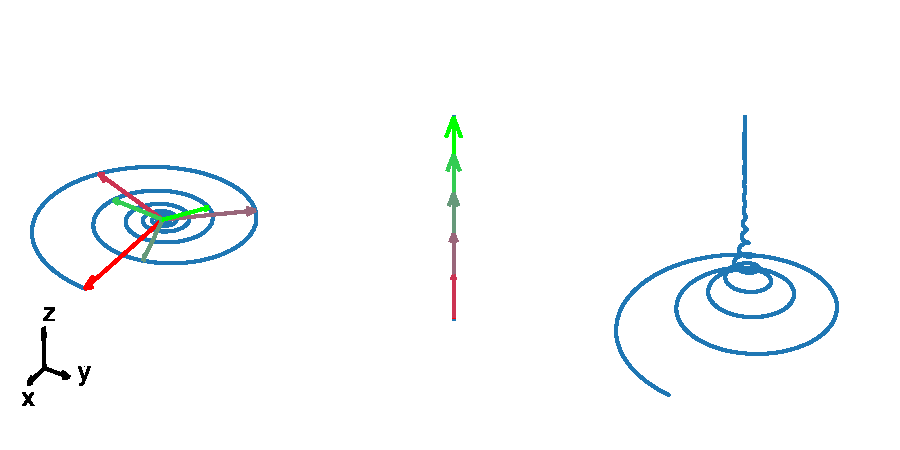
\includegraphics[width=0.9\textwidth]{/figures/theory/relaxation.pdf}
                \caption[Relaxation in NMR]{Exemplary plots of the T$_1$ and $T_2^*$ relaxation after a \SI{90}{\degree} FA shown via the magnetization and its temporal development. On the left, the magnetization in the xy-plane is shown with six arrows indicating equal time-steps. In the center, equal time-steps for the z-magnetization are shown. On the right, both cases are combined to show the overall magnetization. Note that generally, T$_1$ is larger than $T_2$ (here a factor of 10 difference).}
                \label{theory:figure:relaxation}
            \end{figure}
        Macroscopically, the equation
        \begin{equation}
        \frac{dM_{x,y}}{dt} = - \frac{M_{x,y}}{T_2^*}
        \end{equation}
        is solved, a mono-exponential signal decay described by its time constant $T_2$:
        \begin{equation}
            M_T(t) = M_0\exp{\left(\frac{-t}{T_2^*}\right)}
        \end{equation}
        The parameters are mostly derived experimentally, but especially T$_2$ can be - and often is - theoretically estimated \cite{kaupp_calculation_2003}.
        If multiple RF pulses follow each other, a so-called steady state can be induced.
        In the steady state, the magnetization follows the same path within each TR. That means that, for each repetition, the magnetization starts with the same initial state due to the interplay of RF pulses, gradients and relaxation. Usually, the steady state is not reached until a few repetitions into the sequence. Choosing the right combination of TR and FA\footnote[1]{so-called Ernst angle}, the overall signal per time can be maximized \cite{nitz_contrast_1999}.
        \subsection{Inversion recovery}
        T$_1$ times of a sample can be measured using so-called inversion recovery experiments. The measurement is usually implemented by a \SI{180}{\degree} pulse inverting the longitudinal magnetization followed by a \SI{90}{\degree} pulse. The RF pulses are separated by an evolution time $t_{ev}$ during which the z-magnetization recovers. t$_{ev}$ is varied over the course of the experiment. For each set of \SI{180}{\degree} and \SI{90}{\degree} pulse and evolution time, one point of the z-magnetization is sampled. Alternatively, the \SI{90}{\degree} RF-pulse can be replaced by many, smaller flip angle pulses generating much less signal than a \SI{90}{\degree} pulse as shown in figure \ref{figure:theory:inversionRecovery}, right. Sampling intervals are now shorter than the previous evolution times. The additional change in z-magnetization generated by each pulse has to be considered in the calculation of T$_1$, the z-magnetization can be described by:
        \begin{equation}
            \begin{split}
                M_{z,n} =& \\ &M_0 \left(1-\exp{\left(\frac{T_R}{T_1}\right)}\right)\frac{1-\cos(\alpha)^n\exp\left(\frac{T_R}{T_1}\right)^n}{1-\cos(\alpha)\exp\left(\frac{T_R}{T_1}\right)}\\ 
                         &+M_{0,z}\cos(\alpha)^n\exp\left(\frac{T_R}{T_1}\right)^n
            \end{split}
        \end{equation}
        where $M_{0,z}$ is the polarization after the inversion pulse and $M_0$ is the equilibrium polarization \cite{look_time_1970-1, drobnitzky_closed-form_2017}.
            \begin{figure}
                \centering
                \includegraphics[width=\textwidth]{/figures/theory/saturationRecovery.pdf}
                \caption[Saturation recovery]{Saturation recovery sampling schemes. Left, the standard scheme is displayed. An inversion pulse is followed by a readout pulse after an inversion time t$_{inv}$. One evolution time samples one point on the magnetization curve. The experiment has to be repeated multiple times for different inversion times. On the right, a faster scheme using smaller FAs and only a single inversion is shown in which multiple points along the inversion curve are sampled in one experiment.}
                \label{figure:theory:inversionRecovery}
            \end{figure}
            For non-uniform samples where the relaxation constants differ over the sample distribution, multiple T$_1$ values corresponding to different volumes can be acquired for different using spatial encoding (see \cite{scheffler_t1_2001} / sec. \ref{sec:theory:magneticGradient}).
            \subsection{Spin echoes}
            \label{sec:theory:spinEchoes}
            As previously described, T$_2^*$ is shorter, often - especially for inhomogeneous samples - even substantially smaller than T$_2$. Dephasing of the transverse magnetization is thus faster than for a pure T$_2$ decay. A so-called refocusing pulse can be inserted  behind the excitation pulse after a time t$_e/2$. The refocusing pulses are \SI{180}{\degree} pulses now acting on the transversal magnetization\footnote[1]{Note that the inversion pulses act on both longitudinal and transversal magnetization, but only the latter is of relevance here.} of each nucleus which is rotated by \SI{180}{\degree} around the B$_1$ axis of the pulse. Considering the nuclei as spatially static within the temporal scope of the pulse sequence, the dephasing induced by macroscopic field inhomogeneities will be recovered at a time t$_e$ after the excitation pulse. The constructive overlay of the spins forms an observable signal called spin echo.
            This scheme is not limited to a single echo, but multiple inversion pulse can be used to create an echo train. The maximum signal in each echo corresponds to the pure T$_2$ signal envelope.
            %\subsection{2D-NMR}
            %\label{chapter:theory:2DNMR}
         %As the standard NMR spectrum can get difficult to interpret when many different or large molecules are present and many nuclei at different freqencies contribute to the signal, 2D-NMR methods were invented. A method called COSY emerged in 1976, the simplest and most widely used 2D-NMR method on which many other sequences are based  \cite{spie_ad_1982-1}. The second dimension that is added is created by multiply recording a 1D spectrum, but continuously varying a parameter for each measurement. This is mostly an evolution time t$_e$. The variation of t$_e$ corresponds to a secondary sampling and is plotted as the second dimension after an additional fourier transformation of the recorded spectra. \cite{finster_two-dimensional_1980}. In COSY, where both dimensions are sampled equivalently, the diagonal peaks correspond to those in the 1D NMR spectrum whereas off-diagonal peaks show couplings between different nuclei.
         %More advanced 2D NMR methods can also help measuring couplings between different nuclei such as $^1$H and $^{13}$C or to resolve J couplings more easily.

         %The method is very similar to the MRI method described in chapter \ref{sec:theory:MRI} although here, no field gradients are necessary yet: the second dimension simply shows the development of certain nuclei's signals under a specific interaction during a varying evolution time that is defined by the pulse sequence.
        \subsection{Magnetic field gradients}
            \label{sec:theory:magneticGradient}
            For a spatial distinction of the origin of a NMR signal, it is beneficial to not only have the homogeneous $B_0$ field, but to also introduce magnetic field gradients. Generally, these are additional fields ideally oriented exactly along the primary magnetic field's direction that change with one of the x, y and/or z spatial dimensions \footnote[2]{The naming convention calling the gradient an x-gradient does not imply a field in x direction.}. The most common, minimum requirement for imaging are linear gradients, i.e. fields that in- or decrease linearly with one spatial direction. More complex magnetic field gradients \cite{littin_development_2018} are mostly used for shimming \cite{kim_regularized_2002} but also for advanced imaging sequences such as radial sequences like the 'stack of stars' sequence \cite{burdumy_one-second_2016}. Generation of magnetic field gradients is usually achieved through normal conductors of specifically tailored geometries. Gradient strengths and ramping speeds are limited by the specific absorption rates (SAR) that are defined by the IEC standard \cite{noauthor_iec_nodate} as spatially or temporally quickly changing magnetic fields can cause neuronal stimulation in living tissue. 
    \section{Magnetic Resonance Imaging (MRI)}
        \label{sec:theory:MRI}
        A huge addition to the world of NMR was the invention of spatially resolved sample maps, i.e. imaging. It was made possible through the clever use of magnetic field gradients which allow to differentiate between signals of different spatial origin (see also section \ref{sec:theory:magneticGradient}).
        As a non-invasive, non-ionizing imaging method, MRI has become important in many parts of the medical field for example neurology \cite{frisoni_clinical_2010}, oncology \cite{padhani_dynamic_2002} or cardiology \cite{constantine_role_2004}. While MRI methods are limited by the rather low polarization of nuclei (on the scale of $10^{-5}$), the contrasts available differ vastly from other methods. This allows for imaging of unique tissues contrasts and physiological processes inaccessible through other means. In the following, a basic imaging sequence is described \cite{noauthor_wiley-vch_nodate}.
        \subsection{Spatial encoding}
            To describe an image, it is convenient to introduce k-space, which is the 2D\footnote[1]{or, if the recording is in three dimensions, 3D}-Fourier transform of an image. The k-space can be used to describe the sampling schemes applied in many sequences and the inverse FT of a correctly sampled k-space will generate the image of interest.
        \subsubsection{Magnetic field gradients}
        To generate an image of a subject inside the magnetic field, the spatial origin of the NMR signal described in the previous sections must be determined. As the signal in a homogeneous field is independent of an objects position, field gradients are introduced. A perfect x-gradient, for example, has magnetic components along the z-direction only which vary linearly with the x-position. As described before (sec. \ref{sec:theory:magneticGradient}), these field gradients are used for shimming, but also for spatial encoding of the NMR signal. The latter is described in more detail in the following. The gradient fields used for spatial encoding are typically several orders of magnitude higher compared to those for shimming. Imaging sequences consist of RF pulses, magnetic field gradients and readout - all arranged and sequenced in an application specific manner.
        \subsubsection{Slice selection}
        \label{sec:theory:sliceSelection}
        In order to acquire a two-dimensional image, first a slice has to be selected at the desired location. To do so, a magnetic field gradient is applied to the sample. 
            \begin{equation}
                B_z(z) = B_{z,max} \cdot \frac{z}{z_{max}}
            \end{equation}
            For convenience, the slice selection direction is usually labelled to be along the z-direction, although z does not necessarily coincide with the z-direction in the laboratory frame but can be oriented in any direction.
            The slice thickness $\Delta$z is defined by the gradient strength and the frequency bandwidth of the RF-pulse:
            \begin{equation}
                \Delta f = \gamma G_z \Delta z
            \end{equation}
            where $G_z$ is the gradient strength in \si{\tesla\per\meter}.
            Radiofrequency pulses have a limited frequency bandwidth which is inversely proportional to their duration, but changes with the pulse shape. Thus, with the z-gradient turned on, they will affect only nuclei within a slice of the thickness defined by
            \begin{equation}
                \Delta z = \Delta f_{pulse} \cdot \frac{1}{\gamma G_z}.
            \end{equation}
             The following pulses in the sequence have to be carefully designed to not generate FIDs or echos of their own that are not related to the originally selected slice. So called crusher gradients can be used to dephase the remaining coherences so strongly that they will not contribute to following readouts.
        \subsubsection{Frequency encoding}
        A field gradient called readout gradient can be turned on before readout to encode the second spatial dimension. Considering a gradient in the x direction (not necessarily along one of the scanner coordinate system axes), the nuclei at higher x values will then possess a higher frequency than the ones at lower x values.
            \begin{equation}
                f(x) = \gamma B_0 + \gamma G_x \cdot x
            \end{equation}
              By sampling the signal and Fourier transforming it, a projection of the previously excited slice (sec. \ref{sec:theory:sliceSelection}) onto the x-axis is generated. In k-space, the signal acquisition corresponds to the sampling of one line running through the center of k-space.
        \subsubsection{Phase encoding}
            Generating an encoding for the third spatial dimension is not quite as straightforward.  To do so, a third gradient in a third dimension perpendicular to the two others, a y-gradient, is necessary.  It is used to change the phase of the signal the nuclei generate depending on the y-position in the sample prior to the application of the readout gradient. The additional phase depends on gradient strength and the duration it is switched on:
            \begin{equation}
                \phi = \gamma G_y t
            \end{equation}
            That means that the gradient strength needs to be varied to satisfy the sampling conditions for the frequencies generated, i.e. the frequency encoding scheme (sampling one line in k-space) is run multiple times with different phase encoding gradient field strengths set up run before it. That way, if the Fourier transformed data for each phase encoding step, i.e. each frequency encoded line, is sorted by gradient strength and Fourier transformed in the second dimension, the frequency generated by the changing phase will indicate the position in y direction. That means that each phase encoding step shifts the k-space line in the $k_y$ direction. The gradient is varied stepwise until all lines in k-space have been acquired.
            \begin{figure}
                \includegraphics[width=0.9\textwidth]{/figures/theory/imagingScheme.pdf}
                \centering
                \caption[k-space Graph]{An abstract visualization of an imaging sequence. On the left, the gradients in frequency and phase encoding gradients are displayed over the course of one phase encoding step. For each of these steps, the phase encoding gradient's strength is varied. The usual display of the encoding steps in k-space is displayed on the right. Each repetition of the scheme on the left corresponds to one line in $k_x$ direction on the right shifted in $k_y$-direction by the phase encoding gradient.}
                \label{figure:theory:MRIScheme}
            \end{figure}
            Figure \ref{figure:theory:MRIScheme} illustrates the gradients switched on before and during acquisition. Note that slice selection and RF pulses are not depicted here. Each of the 16 steps shown on the right is executed serially to sample all phase encoding gradients.
        \subsection{Signal generation}
        After excitation of the sample spins and k-space encoding previously described, the sample signal needs to be recorded. To do so, both spin- and gradient echos can be used. The general principle is the same for both - a previously dephased signal is rephased. The basic principle and timings differ though and are described here. 
        \subsubsection{Spin echo sequence}
            As described in section \ref{sec:theory:spinEchoes}, in a MR experiment, after initial RF excitation, spin echoes can be generated. RF inversion pulses usually spaced with a specific echo time TE/2 are used generate the echoes. This means that the time limiting factor for each signal acquisition is $T_2$. Generally, after a single excitation, multiple echoes can be recorded using multiple inversion pulses. It has to be considered that the signal is getting lower with each refocussing according to T$_2$; if T$_2$ is known, this can be accounted for. The refocusing pulse will invert z-magnetization, therefore, in spin-echo sequences, a repetition time TR which is in the order of the longitudinal relaxation time T$_1$ should be used between successive excitations.
        \subsubsection{Gradient echo sequence}
        \label{sec:theory:gradientEcho}
        A gradient echo sequence uses an radiofrequency pulse to generate the initial x-y-magnetization, but relies on additional gradients instead of RF-pulses to actively de- and rephase the magnetization after excitation \cite{brown_mri_2005}. This scheme is faster than the previously described spin echo schemes because it does not require a refocussing pulse and therefore magnetization stays close to thermal equilibrium for small excitation flip angles. This is a huge advantage as the overall sequence durations can be reduced.
        \subsubsection{Steady state sequences}
        In reality, to keep sequence durations low, it usually is not reasonable to wait for complete relaxation in between repetitions. Therefore, imaging sequences work on the steady state principle described in chapter \ref{chapter:theory:relaxation}.
        \subsubsection{Relaxation weighting}
        \label{sec:theory:relaxation}
        The signal that is recorded in a sequence is largely influenced by the relaxation times of the sample measured due to the finite length of pulses and additional delays between pulse and readout. The sequences can be adapted so that the different relaxation times' influence on the overall signal varies. Table \ref{tab:theory:relaxationWeighting} shows the Relaxation constant mainly contributing depending on the sequence timings.
        \begin{table}
            \centering
            \begin{tabular}{|c|cccc|}
                \hline
                TR & short & short & long & long \\
                TE & short & long & short & long \\
                \hline
                weighting  & T$_1$ & - & $^1$H density & T$_2$ \\
                \hline
            \end{tabular}
            \caption[Relaxation weighing]{Influence of repetition and echo time TR and TE on the effective signal recorded in an imaging sequence. Note that in any constellation, both relaxation times will have an effect on the signal, but the dominating relaxation constant is indicated.}
            \label{tab:theory:relaxationWeighting}
        \end{table}
        A short TE will reduce the influence of T$_2$ as the ADC will turn on before strong transversal signal decay occurs. A long TR will reduce the T$_1$ influence on the signal as relaxation towards thermal equilibrium magnetization during the repetition time diminishes the magnetization differences. Using imaging sequences reducing both effects, i.e. with short TE and long TR results in so-called proton or proton density weighted images where the number of proton nuclei within each voxel generates the main contrast. The combination of long TR and long TE will produce a image weighted by the T$_2$ times in the sample and the opposite, long TE and short TR will emphasize the T$_1$ values of the different realms.
        \subsection{Adiabatic field cycling}
        To generate more signal while keeping some advantages of a low field like higher absolute homogeneity, pre-polarization can be used. A magnetic field that is larger than the readout field is switched on for a certain time before the actual measurement. The duration of the pre-polarization field is largely influenced by the T$_1$ times in the sample. The switching times of the fields have to be adapted to the conditions of the setup. If the magnetic fields to be switched between are aligned, the field can be switched off quickly. If there is no alignment, the field must be switched off slowly enough if the magnetization is to follow the changing field direction. This is called adiabatic cycling. Therefore, after the field cycling procedure, an RF-excitation pulse is needed to generate observable signal. Adiabatic here means that the field direction changes about an angle $\phi$ for which the relative rotation of the field is small, i.e. 
            \begin{equation}
                \sin(\phi) B_0 << B_0
            \end{equation}
            within the correlation time of a spin, i.e. within the time it needs for one full precession.
    \section{Hyperpolarization}
    \label{sec:theory:HP}
        The main limitation of NMR and MRI is the low thermal polarization at room temperature at the currently available magnetic field strengths. The population of the spin states follow the Boltzmann distribution \cite{canet_para-hydrogen_2006} which, for each energy state $E_i$ and its corresponding occupation number $N_i$, dictates
        \begin{equation}
            N_i = N \cdot\frac{\exp{\frac{E_i}{k_B T}}}{\sum_n\exp{\frac{E_n}{k_BT}}}
        \end{equation}
        For energy differences between two states of energies $E_+$ and $E_-$ that are small compared to the thermal energy, the polarization can be expressed as follows:
        \begin{equation}
            P = \frac{N_+-N_-}{N} \approx \tanh\left(\frac{\hbar \gamma B}{2 k T }\right)
            \label{equation:theory:polarization}
        \end{equation}
        This means, that even at the relatively high field strengths that can be generated in the spectrometers and MR imagers (order of \SI{10}{\tesla}), only a small fraction of the spins effectively contribute to the overall signal. Figure \ref{figure:theory:boltzmannDistribution} shows this schematically for full polarization. Note that the size of the energy splitting compared to the total energy differs by five orders of magnitude. In clinically relevant MRI machines that mostly operate at \SI{1.5}{\tesla} or \SI{3}{\tesla}, that means that a maximum of 1 in $10^5$ nuclei (at \SI{3}{\tesla}) effectively contributes to the signal.
        \begin{figure}
            \centering
            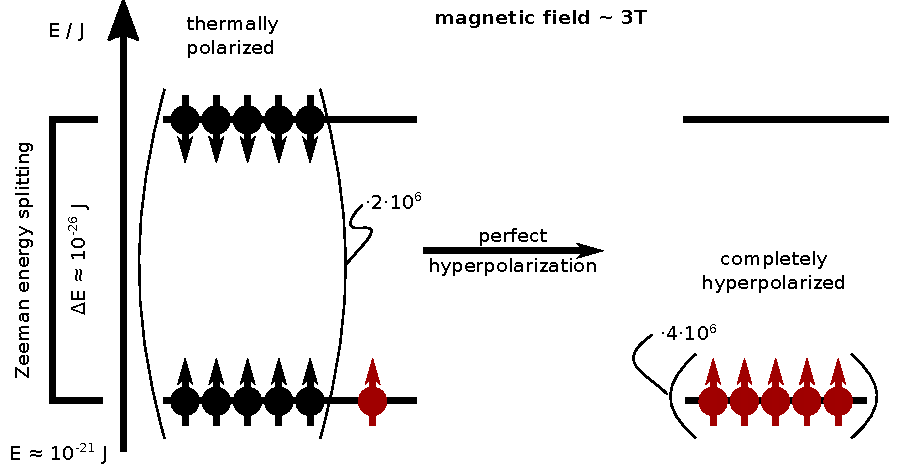
\includegraphics[width=0.9\textwidth]{/figures/theory/hyperpolarizationScheme.pdf}
            \caption[Hyperpolarization scheme]{Hyperpolarization can provide the means to drop all, or at least a lot more than in the thermally polarized case, of the spins to the lower energy level. That way, the overall magnetization and thus the signal observed is a lot higher than in there thermally polarized case. The graph shows the case of perfect hyperpolarization of $^{1}$H at \SI{3}{\tesla}, which of course does not represent reality. At the fields currently used in clinical routine, only about one in 100000 spins effectively contributes to the signal.}
            \label{figure:theory:boltzmannDistribution}
        \end{figure}
        \subsection{Dynamic nuclear polarization}
        As the gyromagnetic ratio of electrons is much higher than that of any nucleus (factor of $10^{3}$ compared to protons), dynamic nuclear polarization (DNP) uses electrons at low temperatures and high fields to generate large initial electron polarization \cite{berliner_spin_1976}. The polarization is then transferred to specific nuclei by microwave irradiation at the electron spin resonance frequency \cite{bajaj_dynamic_2011} of free electrons which are introduced by the addition of free radicals and which provide an unpaired electron spin that couples to the nuclear spins by dipolar coupling. The low temperatures usually required for DNP lead to a freezing of the sample and microwaves are applied to it in that frozen state. For administration to a specimen or patient, the frozen sample then needs to be quickly melted and transferred \cite{johannesson_dynamic_2009}, usually in controlled magnetic environments \cite{milani_magnetic_2015} to prevent fast relaxation. The samples can show high polarization close to unity but the measured signal enhancement is usually limited by decay during the relatively long delivery times. Efforts building faster transport mechanisms have greatly reduced these times but they remain in the range of tens of seconds.
        \subsection{Hyperpolarization of noble gases}
        Noble gases such as 3He or 129Xe can be hyperpolarized by optical pumping \cite{middleton_mr_1995,oros_hyperpolarized_2004}. To do so, usually lasers are focused onto an optical cell through which the gas flows. The hyperpolarization is induced via the polarization of electron spins. An alkali metal, often Rubidium \cite{hersman_large_2008}, serves as a receptor for the laser induced optical pumping and subsequently hyperpolarizes the nuclei of the noble gas by spin exchange interactions \cite{walker_spin-exchange_1997}. Hyperpolarized gases are primarily used in lung imaging, but other uses e.g. in liquid state NMR or MRI by gas dissolution are not precluded \cite{duhamel_xenon-129_2001}.
        \subsection{Brute force hyperpolarization}
        As equation \ref{equation:theory:polarization} indicates, there are two main factors influencing polarization: magnetic field and temperature. It is not an option to freeze the objects to be measured, as strong polarization effects occur only close to absolute zero temperatures at the magnetic fields that can currently be generated. A viable alternative is to hyperpolarize a tracer cooled to \si{\milli\kelvin} temperatures (and thus frozen) at high fields, wait until polarization has built up, thawing it and administering it to the subject \cite{hirsch_brute-force_2015}. Here, in contrast to DNP, no free radicals are necessary to generate the HP and - depending on the relaxation constants in the field and temperature regime - no or less harmful additives than the free radicals for DNP are necessary. This makes a faster and lossless transfer of the sample to the subject possible. The high polarization generated on $^{1}$H can then be transferred to x-nuclei e.g. by passing the sample through low fields (< \SI{10}{\milli\tesla}). The transfer is driven by thermal mixing \cite{goldman_overview_2008} of the two spin species. Brute force hyperpolarization is limited by the extremely long T$_1$s at ultra low temperature which leads to exceedingly long polarization times.
        \subsection{Parahydrogen induced hyperpolarization (PHIP)}
            Hydrogen is a spin 1/2 particle and thus underlies the Fermi-Dirac statistics. Its angular momentum is described by the nuclear angular moments and the rotational angular momentum. Hydrogen molecules occur in one of the four spin states
            \begin{equation}
                 \begin{aligned}
                     T_+ &=\ket{1,1} & = & |\uparrow\uparrow\rangle\\
                     T_0 &= \ket{1,0} & = &\frac{1}{\sqrt{2}}\left(|\uparrow\downarrow\rangle + |\downarrow\uparrow\rangle\right)\\
                     T_- &= \ket{1,-1}& = & |\downarrow\downarrow\rangle\\
                     S &= \ket{0,0} & = &\frac{1}{\sqrt{2}}\left(|\uparrow\downarrow\rangle - |\downarrow\uparrow\rangle\right)
                 \end{aligned}
            \end{equation}
            where T indicates the triplet state with overall spin I = 1 and S the singlet state with I = 0. Parahydrogen is the singlet state of the hydrogen molecule, i.e. the antisymmetric mixed up/down state. The molecules spin states are coupled to their rotational states. At room temperature, the even and odd rotational states are almost equally occupied which in turn means that the four spin states are also almost equally occupied as thermal energy is large compared to rotational energies of the molecule \cite{green_theory_2012-1}:
            \begin{equation}
                \frac{N_{para}}{N_{ortho}} = \frac{\sum_{J=even}(2J+1)\exp\left(-\frac{J(J+1)\Theta_R}{T}\right)}{3\sum_{J=odd}\left(2J+1\right)\exp\left(-\frac{J(J+1)\Theta_R}{T}\right)}
            \end{equation}
            where J is the rotational quantum number, $\Theta_R$ is the rotational energy constant of parahydrogen \cite{noauthor_orthohydrogen_1935}. At high temperatures, the exponential terms approach 0 and the ratio converges towards $\tfrac{1}{3}$. That means that compared to the thermal energy, the rotational energies can be neglected to a good approximation at room temperature. Approaching absolute zero, the fraction of pH$_2$ rises towards the pure pH$_2$ state as the denominator approaches zero (see figure \ref{figure:theory:ph2Fraction}). At temperatures used to generate parahydrogen in this work, around \SI{21}{\kelvin}, the pH$_2$ fraction is close to 1 with about \SI{98}{\percent} parahydrogen fraction.
            The conversion of oH$_2$ to pH$_2$ and back is forbidden quantum mechanically due to the necessary change in spin angular momentum (0 to 1) that would change the symmetry of the wavefunction (Pauli principle)\cite{minaev_spin_1995}. Therefore, conversions are only possible if different molecules collide and their nuclei interact or if the magnetic momentum of the rotating molecule interacts with the nuclear moments, which is both improbable and thus slow. Theoretical lifetimes in neat gas are in the range of years \cite{green_theory_2012-1}, though in reality, e.g. through interaction with vessel walls, these long lifetimes reduce to the order of days. As the transition is forbidden in both directions, to be able to generate pH$_2$ fast and in large quantities, additional interactions need to be introduced that catalyzes the conversion. Both charcoal catalysts and iron oxide have been proposed \cite{dechent_proton_nodate}. The catalyst creates field gradients on the scale of the hydrogen molecule which enables spin mixing of ortho and para states\cite{minaev_spin_1995} and thus a much faster conversion. This means that, at liquid helium temperatures which were used in this work, parahydrogen can be enriched to almost \SI{100}{\%}, a liquid nitrogen generator would enrich it to about \SI{50}{\%} \cite{zhuzhgov_low-temperature_2018}.
            As parahydrogen itself is a spin 0 particle, it is MR-invisible. Its ordered state can be used though to polarize other molecules, often referred to as substrate molecules or target molecules.
            \begin{figure}
                \centering
                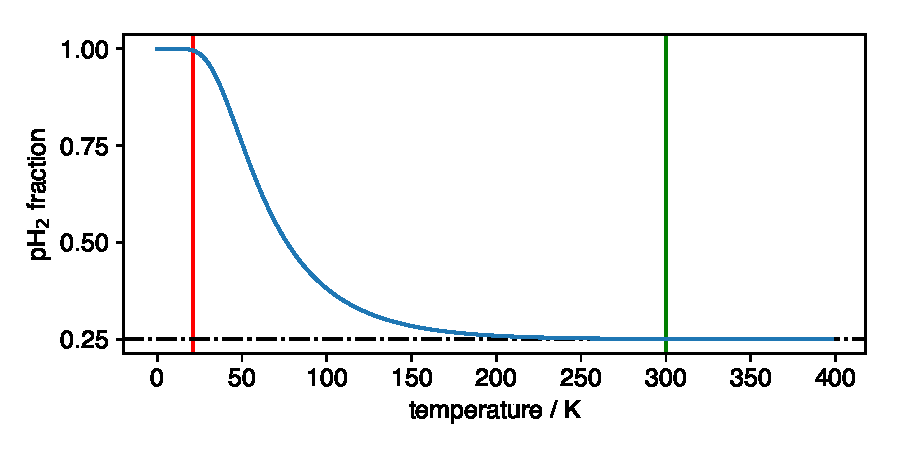
\includegraphics[width=0.9\textwidth]{/figures/theory/parahydrogenFraction.pdf}
                \caption[Parahydrogen fraction]{The equilibrium population of the para hydrogen state. The dashed line shows the high temperature limit of 3:1. The green line indicates room temperature, where the limit is almost reached. The red line indicates the temperature at which parahydrogen was generated in this work, \SI{21}{\kelvin}.}
                \label{figure:theory:ph2Fraction}
            \end{figure}
            The initial density matrix of parahydrogen can be described by
            \begin{equation}
                \sigma_0^{pH_2} = \frac{1}{4} \hat 1 - c_0(\hat{I}_1\hat{I}_2)
            \end{equation}
            with the individual spins' operators denoted by 1 and 2 \cite{green_theory_2012-1} and the constant $c_0$ scaling with the fraction of $pH_2$ in the initial gas mixture:
            \begin{equation*}
                c_0=(4f_p-1)/3.
            \end{equation*}
            The evolution of the states is then described by the evolution of the density matrix under the J couplings and chemical shifts in the target molecule and other surrounding nuclei. 
        \subsubsection{Pasadena \& PHIP}
        The first parahydrogen induced polarization (PHIP) experiments were performed at the CIT in Pasadena \cite{bowers_parahydrogen_1987-2}, and later named after it (Pasadena/Altadena). These experiments used parahydrogen to hydrogenate a molecule first and then utilized pulse sequences or field shuttling to generate observable magnetization from the parahydrogen singlet state (broken by the two distinct couplings in the molecule). Later, polarization was also transferred to nuclei other than $^{1}$H. Mostly, $^{13}$C-labeled molecules were used as recipients of the spin order and subsequent polarization. Figure \ref{fig:theory:pasadena} visualizes the hydrogenation of fumaric acid to pyruvic acid. Polarization transfer to the $^{13}$C atom with which the molecule was previously labeled would follow the hydrogenation.
        \begin{figure}
            \centering
            \includegraphics[width=0.99\textwidth]{/figures/theory/pasadena.pdf}
            \caption[Pasadena hyperpolarization]{Hydrogenation scheme used to hyperpolarize the $^{13}$C labeled (*) fumaric acid (a) through hydrogenation with parahydrogen to pyruvic acid (b). The spin order is then converted into polarization on the labeled atom in the molecule (c).}
            \label{fig:theory:pasadena}
        \end{figure}
        To make hyperpolarization possible, the parahydrogen needs to be added to the molecule pairwise, but have to be magnetically distinct after addition \cite{eisenberg_parahydrogen-induced_1991}. That means that after the addition, the symmetry of the added hydrogen molecule must be broken to be able to transfer the spin order. This usually happens already through the asymmetry of the receptor molecule and the different couplings or chemical shifts of each added hydrogen atom of the molecule. Recently, the method has been extended and is now also used to hyperpolarize molecules that are more biologically relevant such as $^{13}$C labeled pyruvate \cite{cavallari_metabolic_2019}.
        \subsubsection{SABRE hyperpolarization}
        \label{sec:theory:HPSabre}
        The signal amplification by reversible exchange (SABRE) method was developed in 2009 \cite{adams_reversible_2009-2} for pyridine as a substrate and an Ir-based catalyst.
        In SABRE, the molecule to be hyperpolarized is not hydrogenated, but is in contact with parahydrogen via the Ir-based catalyst, $\mathrm{IrH_2(COD)(PCy_3)(MeCN)}$, often referred to as IrIMes, for a certain contact time $t_c$. The transfer of spin order can happen spontaneously at the right fields \cite{atkinson_spontaneous_2009-1} where so called level-anti-crossings (LACs, sec. \ref{sec:theory:LAC}) occur. In addition, hyperpolarized substrate can also be generated at fields far from these LACs using RF-irradiation \cite{pravdivtsev_spin_2014, knecht_quantitative_2019} and can also be enriched using selective pulse sequences \cite{knecht_re-polarization_2018-1}. The system can be described by time evolution periods in bound and unbound state, respectively, where the bound state implies non-zero couplings between pH$_2$ and at least one of the substrate spins.
            \begin{figure}
                \centering
                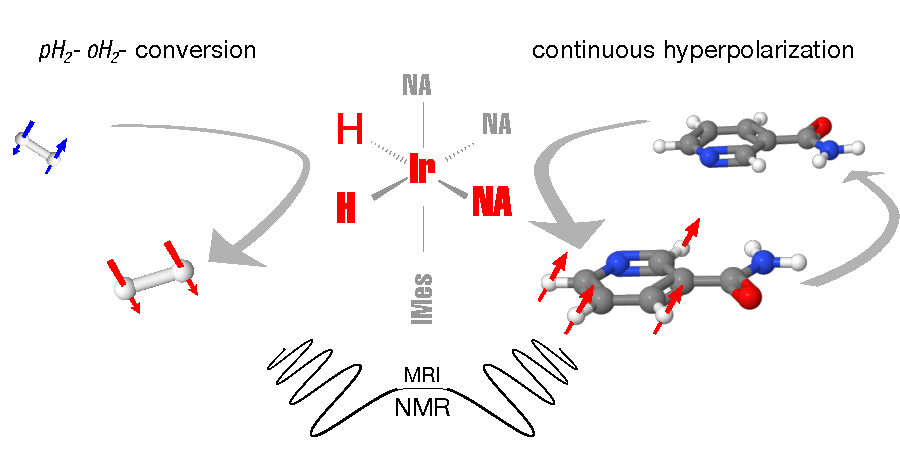
\includegraphics[width=0.9\textwidth]{/figures/theory/sabreScheme.pdf}
                \caption[SABRE scheme]{The mechanism of SABRE using nicotinamide as an exemplary molecule. On the left, parahydrogen is converted to its ortho state. On the right, nicotinamide is hyperpolarized. Centrally, a simplified chemical structure of the catalyst is shown. Figure taken from \cite{rovedo_molecular_2016}.}
            \end{figure}
            To describe the time evolution of the bound system, the density matrix has to be evolved under the couplings present in the complex that forms when both parahydrogen and substrate are bound to, and thus coupled via, the catalyst \cite{cowley_iridium_2011-1}. The necessary Hamiltonian is formed by the Zeeman term and all the relevant couplings:
            \begin{equation}
                \begin{aligned}
                    \mathcal{H}& = \mathcal{H}_z + \mathcal{H}_J \\
                        & =\-2\pi\gamma B_0 \sum_n{(1-\delta_n)\hat{I}_{nz}} + \sum_{n<m} -2\pi J_{nm}(\hat{I}_{nx}\hat{I}_{mx} + \hat{I}_{nx}\hat{I}_{mx}+ \hat{I}_{ny}\hat{I}_{my} + \hat{I}_{nx}\hat{I}_{mx})
                \end{aligned}
            \end{equation}
            The binding time that depends on temperature and diffusion constants of the solvent has a strong influence on the effectiveness of the polarization process. Using the time evolution of the Hamiltonian, optimal time values can be found for different settings.
            Hyperpolarization occurs at different points in the system: The substrate itself is hyperpolarized, in both its bound and free form, i.e. after detaching from the catalyst. These forms can be differentiated by their different chemical shifts. At common concentrations, where a excess of target substrate is present, the free form will exceed the bound form drastically. Additionally, the hydrogen will be in a ortho state and hyperpolarized after polarization has been transferred to the target molecule. 
        \subsubsection{$^{15}$N SABRE}
        \label{sec:theory:15nSabre}
        To hyperpolarize $^{15}$N nuclei using SABRE, other energy matching conditions than for hydrogen nuclei have to be fulfilled. As the Larmor frequency differences of the protons carrying the spin order and the nitrogen are much larger than in the pure proton classical SABRE, the fields to match the energies have to be much smaller:
        \begin{equation}
            J_{HN} = \nu_H - \nu_B
        \end{equation}
        where $\nu_H$ and $\nu_N$ are the proton and nitrogen Larmor frequencies and $J_{HN}$ is the effective coupling term \cite{truong_15n_2015-1}. Therefore, fields in the range of \SI{100}{\nano\tesla} are necessary to hyperpolarize $^{15}$N.
        \subsection{Level anti crossings}
        \label{sec:theory:LAC}
        The effect the SABRE method is based on, can be explained by observing the populations of two energy levels magnetic fields around a point of degeneracy. When coupling between the nuclei leads to a deviation from the pure Zeeman energy levels, the so called level anti crossings (LACs) or avoided crossings. In the uncoupled case, two energy levels  can cross at a certain magnetic field strength, i.e. the two states would have the same energy at that point \cite{ivanov_role_2014-2,pravdivtsev_spin_2014}:
        \begin{equation}
            E_0 = E_1 \mathrm{~~\rightarrow~~} \bra{0}H\ket{0} = \bra{1}H\ket{1}
        \end{equation}
        If the nuclei are coupled though, the crossing is avoided and there is a defined energy difference between the nuclei's states in the central region of the avoided crossing; the size is determined by the strength of the coupling. Figure \ref{figure:theory:LAC} shows such a crossing for two states crossing in the uncoupled case (red stripes), but avoiding that crossing in the coupled case by $J_{12}$. The Hamiltonian of the system is
        \begin{equation}
            H = \left [
                \begin{array}{ll}
                    E_{1} & W_{12}\\
                    W_{21} & E_2
                \end{array}
            \right ]
        \end{equation} 
        where $W_{12}$ is the coupling between the energy levels $E_1$ and $E_2$ which leads to new eigenenergies
        \begin{align*}
            E_+ &= \frac{1}{2} \left[(E_0+ E_1) + \sqrt{(E_0-E_1)^2+4|W_{12}|^2}\right]\\
            E_- &= \frac{1}{2} \left[(E_0+ E_1) - \sqrt{(E_0-E_1)^2+4|W_{12}|^2}\right]
        \end{align*}
        which, for $W_{12}=0$ gives the Eigenstates of the uncoupled system, $E_1$ and $E_2$. The corresponding new Eigenstates are 
        \begin{equation*}
            \ket{+} = \cos\frac{{\theta}}{2}\exp{i\phi}\ket{0} + \sin{\frac{\theta}{2}}\exp{i\phi}\ket{1}\\
        \end{equation*}
        \begin{equation*}
            \ket{-} = -\sin{\frac{\theta}{2}}\exp{i\phi}\ket{0} + \sin{\frac{\theta}{2}}\exp{i\phi}\ket{1}
        \end{equation*}
            \begin{figure}
                \centering
                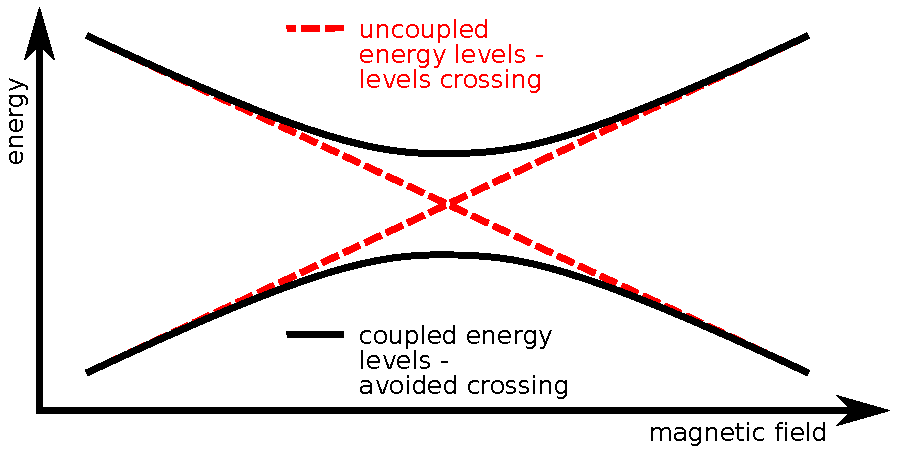
\includegraphics[width=0.9 \textwidth]{/figures/theory/LACs.pdf}
                \caption[Level anti crossings]{A generic example of level anti crossings. In red, the uncoupled states can be seen while in black, the energy states in the presence of coupling are shown.}
                \label{figure:theory:LAC}
            \end{figure}
            This means that the coupling leads to a mixing of the states if the magnetic field, which determines the energy difference between $E_2$ and $E_1$, is in the region of the LAC. Effectively, the coupling thus changes the occupational numbers of the uncoupled states over time. See section \ref{sec:theory:HPSabre} for how this effect can be used to hyperpolarize samples.
        \section{Hardware}
            As hardware plays an important role in this work, I also want to provide a bit of insight into some of the technologies used in this work.
            \subsection{Field generation}
                The magnetic fields are generated by either current flown conductors or superconductors with exception of a few cases where permanent magnets are used. Both normal and superconductors have ad- and disadvantages and are chosen according to requirements (see \ref{chap:MaterialsAndMethods}). Magnetic field is generated according to the fourth Maxwell equation
                \begin{equation}
                    \label{equation:theory:maxwell}
                    \vec\nabla\times\vec B = \mu_0\vec j+\mu_0\epsilon_0\frac{\partial\vec E}{\partial t}
                \end{equation}
                where $\vec j$ is the electric current generating the magnetic field together with changes in the electric field \cite{b.i._bleaney__b._bleaney_electricity_nodate}. For the static field of a conductor, the current is the main mechanism of field generation and is described by the Biot-Savart-law.
            \subsubsection{Normal conductors}
                A normal conductor has the great advantage of room temperature operation, simplifying its setup and use enormously. The disadvantage is  its finite resistance. That means the conductor will generate heat which will limit the maximum current at which it can be safely operated.  That heating can be so large that melting of the conductor occurs or, in the less dramatic case, deformations happen due to heat expansion and/or softening of the conductor material. Usually, copper is chosen for its low electric resistance of \SI{1.72e-8}{\ohm\meter}(reducing heat generation) and at the same time high thermal conductivity \SI{380}{\watt\per\m\per\kelvin}(increasing heat dissipation) \cite{schofield_f._h._thermal_1925}.
            \subsubsection{Superconductors}
            \label{sec:theory:superconductor}
            Superconductors are a special form of conductors that show electric resistances of zero below a certain critical temperature $T_c$ discovered in 1911 \cite{onnes_resistance_1911}. Generally, superconductors need to be cooled to a few \si{\kelvin} to show this property, modern alloys so called high temperature superconductors can, under certain conditions, raise that limit to up to \SI{200}{\kelvin} \cite{drozdov_conventional_2015}. Superconductors can be made of different, rather exotic materials but also more common substances such as graphene can show superconducting properties \cite{cao_unconventional_2018}. Different superconductors show different critical Temperatures and mechanical properties often restricting their use to certain fields. Microscopically, inside the superconductors, so called cooper pairs are forming \cite{bardeen_theory_1957}. These pairs of two electrons travel resistance free through phonon coupling, i.e. the deformation of the surrounding lattice caused by one electron distribution and the related energy loss is regained \SI{100}{\percent} by a second electron. That way, completely lossless movement of electrons is possible in the compound.
            \subsection{Magnetic susceptibility and shielding}
                The magnetic field generated by a current flow or a changing electric field is described by the magnetic field strength $\mat H$ which describes the magnetic field with no material present. The actually relevant size for experimental purposes is the magnetic flux density $B$ which adds to the magnetic field strength the magnetization $M$ of materials exposed to the magnetic field strength $H$.
                \begin{equation}
                    \vec{B} = \mu \vec{H} = \mu_0 \mu_r \vec{H} = \mu_0(1+\chi) \vec{H}
                \end{equation}
                where $\chi$ is the magnetic susceptibility \cite{schenck_role_1996}, the quantity mostly mentioned in NMR and MRI. Usually, $B$ is the quantity intended when talking about magnetic fields.
                In many cases, as for example for air, $B$ and $H$ are almost the same as the relative permeability \cite{kriz_magnetic_1996} $\mu_r$ is only 0.35 ppm \cite{cullity_introduction_2008}. For water, it is already about a factor 10 higher, i.e. $\mu_r$ = 2~ppm . 
                This means that, where susceptibility changes occur in materials, magnetization and thus magnetic field's change. These changes cause field inhomogeneities posing a problem for NMR and MRI where a more homogeneous field ($B_0$) is always preferred. Materials are grouped by their susceptibilities \cite{b.i._bleaney__b._bleaney_electricity_nodate}:
                Substances with a large, positive $\chi$ are called ferromagnetic, they are magnetized in the direction of the external field and the magnetization can surpass the field strength of the external field. External field and magnetization aren't usually linearly correlated for ferromagnets, when all magnetic moments in the material are aligned a plateau is reached. Usually, these materials follow a magnetization hysteresis when the external field changes value and sign. Furthermore, ferromagnets do not necessarily return to their unmagnetized state if H returns to 0 (remanence).
                Paramagnetic and diamagnetic substances show a much smaller magnetization, where paramagnetic substances' electron magnetic moments, as ferromagnetic ones, align parallel to the magnetic field ($\chi>0$) and diamagnetic antiparallel ($\chi$ < 0).
                Shielding of external magnetic fields can make use of the fact that the high susceptibility of some materials leads to a bundling of magnetic field lines, i.e. a volume surrounded by that material can have a strongly reduced magnetic flux density and thus a lower magnetic field \cite{mager_magnetic_1970}.
            \subsection{Oscillating circuit}
                A coil for usage in NMR or MRI usually consists of oscillatory circuits made up of a capacitor of capacitance $C$ and an inductance $L$. Inside a oscillatory circuit, energy can be stored in the forms of electric field and electric current. The two forms of energy are constantly converted into each other, i.e. the capacitor is charged by the current coming from the coil and in turn generates a phase shifted countering current. The frequency of this conversion can be calculated considering the following differential equations:
                \begin{equation}
                    \begin{aligned}
                        -L\frac{dI}{dt} &= \frac{Q}{C} \\
                        L\frac{d^2I}{dt^2} + \frac{I}{C} &= 0
                    \end{aligned}
                \end{equation}
                as the voltages of coil - that is proportional to the change in current according to Faraday's law - and the capacitor - that depends on capacitance and charge - need to be equal at all times. The solution of this simplified case resulting in a ordinary second order differential equation with no linear term is simply a undamped oscillation:
                \begin{equation}
                    I(t) =  A \cdot \cos(\omega t) + \phi 
                \end{equation}
                where $f= \frac{1}{\omega} = \frac{1}{2\pi\sqrt{LC}}$ which means that by changing capacitance and inductance in a resonant circuit, the resulting resonance frequency can be changed \cite{rao_electronic_2011}. Moreover, capacitance and inductance sizes can be adapted in opposite directions depending on the purpose of operation.
                Of course, in realistic cases, the oscillation is dampened by ohmic resistance of the components and radiation losses (Q-factor).
            \subsection{Birdcage coils}
            Commercially available volume resonators are often manufactured in the birdcage design. The design is based on an array of individual resonant circuits, mostly in a bent, rectangular shape called leg where one side of the leg is a conductor shared by the neighboring legs The rotating magnetization induces a current in those legs, the currents in neighboring legs are phase shifted according to the overall number of legs $\phi_{mag} = 360\si{\degree}/n_R$. As the total phase shift over the resonator must be a multiple of 2$\pi$, if all legs' impedances are the same, the coil can be driven and read out at two points only - generating the above mentioned phase shift by itself. Birdcage coils are mostly chosen for transmission. In small animal scanners, they're also used as receive coils in rodents where the diameters of the specimen are close to the coil diameter. In human scanners, where filling factors are often worse, nowadays, mostly multichannel coil arrays are used.
            \subsection{Saddle coil}
            \label{sec:theory:saddleCoils}
            The saddle coil used for RF-excitation of the sample in the low field spectrometer described later (sec. \ref{sec:matMeth:lowFieldSpectrometer}) is designed based on the publication by Hoult, \cite{hoult_signal--noise_1976}. It derives that the field generated by a saddle coil is given by
            \begin{equation}
                B_{xy} = \frac{\sqrt 3 \mu\mu_0}{\pi}\left(\frac{ag}{(a^2+g^2)^{3/2}}+\frac{g}{a(a^2+g^2)^{1/2}}\right)
            \end{equation}
            where a is the radius of the coil and g is half the height. Using these calculations, an optimum field homogeneity is reached when the opening angle of the coil is \SI{120}{\degree} and the length is equal to the diameter of the coil.
            \subsection{Operational amplifiers}
            Operational amplifiers (opamps) have been used to amplify the signal of the fluxgate magnetic field sensor described in section \ref{sec:methodsfluxgate}. Amplification is necessary because of the large output range of $\pm$ \SI{10}{\volt} in combination with the high resolution in the low field regime. Operational amplifiers are a rather complex network of transistors that show a behavior similar to the ideal operational amplifier described in the following. The ideal operational amplifier amplifies the incoming signal to infinity on the positive input, to $-\infty$ on the negative input and has infinite input impedance as well. This is not true in practice, but very high voltages (limited by the supply voltage) are produced at the output if a small voltage is applied to either of the inputs. With the gain $A_{opa}$, the output voltage is thus described by
                \begin{equation}
                        \label{equation:theory:OPAvoltage}
                    U_{out} = A_{opa}(V_+ - V_-)
                \end{equation}
                That is why operational amplifiers need to be driven in some kind of feedback mode (figure \ref{figure:theory:opAmp}) as otherwise even very small voltage differences on the input cause a saturation of the output. In this mode, the output is fed back to one of the inputs, most of the time via resistors, to generate a defined output voltage that depends on the input voltage of the complete setup, $U_{in}$. The so called inverting opamp that was used in this work, is shown in figure \ref{figure:theory:opAmp} and will be described in more detail now.
                \begin{figure}
                    \includegraphics[width=0.9\textwidth]{/figures/theory/opAmp.pdf}
                    \caption[Operational amplifier]{An operational amplifier in an inverting setup. The amplification of the input voltage $U_{in}$ is directly given by the ratio of the resistors, $R_2/R_1$.}
                    \label{figure:theory:opAmp}
                \end{figure}
                By connecting the output to the negative input, a loop is formed in which the voltages add to zero. This tells us that
                \begin{equation*}
                    U_{opa} = U_{out} - U_- = U_{R_2}
                \end{equation*}
                Additionally, as soon as the negative input starts to differ from the positive one, the output reacts and drives it back. That way, there is a virtual ground on the negative input (marked with a red dot in figure \ref{figure:theory:opAmp}).
                This can also be shown by calculating the voltage $U_-$:
                \begin{equation}
                    U_- = U_{in} + U_{R_1} = U_{R_2} + U_{out}
                \end{equation}
                which, considering $R_1$ and $R_2$ are a voltage divider due to the lack of current through the opamp, this can be written as
                \begin{equation}
                    U_{-} = U_{out} \frac{R_1}{R_1+R_2} + U_{in} \frac{R_2}{R_1+R_2}
                \end{equation}
                and, if combined with equation \ref{equation:theory:OPAvoltage}, gives the output voltage
                \begin{equation}
                    U_{out} = -U_{in} \frac{A_{opa}R_2}{R_1+R_2 + A_{opa}R_1}
                \end{equation}
                which, for large $A_{opa}$ present in all operational amplifiers simplifies to the resistor ratio.
                \begin{equation}
                    U_{out} = -U_{in}\frac{R_2}{R_1}
                \end{equation}
                This also makes sense phenomenologically: with this setup, $U_{+}$ and $U_{-}$ are kept at the same level, i.e. the negative input acts as a virtual ground, as the output is fed back to the negative input and any perturbation that causes a differential voltage between the two inputs will regulate itself by applying a corresponding voltage to the negative input until equilibrium is restored \cite{huijsing_operational_2017-1}.
                This is especially helpful as the accuracy of the resistors is the limiting factor of the amplification's accuracy, i.e. by choosing the resistors carefully, the amplification can be set very accurately.
            \subsection{Frequency filters}
            For reducing noise when interested in certain regions of the frequency spectrum only, frequency filters can be used. They differ in the steepness of the cutoff frequency, so-called order, and the transmission efficiency (no Filter is completely lossless at the unblocked frequencies). The easiest frequency filter is just a combination of a capacitor and a resistor or a inductance and a resistor as shown in figure \ref{figure:theory:frequencyFilter}. Using the impedances of inductance and capacitor
                \begin{equation*}
                    Z_C = -i\frac{1}{\omega C}
                \end{equation*}
                \begin{equation*}
                    Z_L = {i\omega L}
                \end{equation*} 
                The output voltage $U_o$can then be described as a function of input voltage $U_{i}$ and these two impedances:
                \begin{equation}
                    U_o = \frac{Z_c}{Z_R + Z_C} U_i
                \end{equation}
                with the signal frequency $\omega$. The cutoff frequency of the filter $f_0$ can then be described for both the RC-filter by
                \begin{equation}
                    f_0^{RC} = \frac{1}{2\pi R C}
                \end{equation}
                and the RL-filters:
                \begin{equation}
                    f_0^{RL} = \frac{R}{2\pi L}
                \end{equation}
                where the arrangement of the components defines whether it is a low or a high pass filter. These filters are the simplest form of frequency filters of first order and show a boundary drop of \SI{20}{\deci\bel} per frequency decade. Higher order filters can be used where more sharply defined cutoff frequencies are necessary but usually come with drawbacks in the linearity of the transmit band especially close to the cutoff frequency (ripple). These can be constructed by combining multiple frequency filters serially or by designing more complex filters such as the Chebyshev filter, a LC filter with n stages. Figure \ref{figure:theory:frequencyFilter} demonstrates the effect of first and second order filters on the signal at different frequencies.
            \begin{figure}
                \centering
                \includegraphics[width=0.9\textwidth]{/figures/theory/frequencyFilters.pdf}
                \caption[Frequency filters]{Transfer function over frequency for the different types of filters mentioned in the text. Cutoff frequencies are shown for the filters. At the frequency value of 10, a first order high and low pass filter are shown for the same cutoff frequency (i.e. same L/C and R values) in purple colors. Further to the right, a shifted first order filter (C/L * 10) and a second order filter are shown in shades of red.}
                \label{figure:theory:frequencyFilter}
            \end{figure}
            \subsection{Flow and flow resistance}
                For estimation of sample transfer times in the hyperpolarization setup setup described in section \ref{sec:shuttlingSystem}, the flow of liquids through thin tubing had to be considered.
                Pressure differences above liquids or in gases create flow from high to low pressure volumes. These flows can be   described as a function of the pressure creating them under simplified conditions by the Navier Stokes equations \cite{sochi_flow_2013}.
                Flow speeds are generally limited by the flow resistance. This resistance is easily described if the flow is through a tube and can be considered laminar. Generally, the volume flow rate Q is given by the Hagen-Poiseuille equation:
                \begin{equation}
                    Q=\frac{p_2-p_1}{R}
                \end{equation}
                where R is the Reynolds number. Using an electrical circuit as a similarly described system, the Reynolds number would correspond to electrical resistance and the pressure difference would be a voltage equivalent. The Reynolds number generally depends on $\eta$, the viscosity of the fluid and the flow resistance of the connecting vessel. For example, for a solid tube of radius r and length l, the Reynolds number is given by \cite{jeffrey_particle_1965}
                \begin{equation}
                    R=\frac{8\eta l}{\pi r^4}
                \end{equation}
                Because of the much lower viscosity of gases that stems from their lower density, gas flow is generally higher than fluid flow at otherwise unchanged conditions.

    % !TEX root = ../thesis_main.tex
\chapter{Materials and Methods}\label{chap:MaterialsAndMethods}
    \section{Parahydrogen generation and quantification}
    Parahydrogen was generated using a coldhead surrounding a chamber of $\mathrm{FeO_4}$ catalyst which was built before the beginning of this work. The setup is positioned on top of the laboratory building's roof for security reasons with the coldhead on the outside and the temperature sensitive equipment on the insisde. Holes were drilled to make the connections for vaccum hoses, sensor cables and pump exhaust.
        \subsection{Coldhead side}
            The coldhead was cooled down to \SI{21}{\kelvin} via a watercooled helium recondenser with a closed helium circuit. The recondenser was operated at full power while a heater was installed to keep temperatures at 21 K. The coldhead was isolated from surrounding warm air by a vacuum chamber pumped down by a rotary vane pump. A sensor attached to the vaccum chamber read pressures to ensure sufficient isolation before switching on the recondenser. Temperature sensors in the catalyst chamber and on top of the coolant line were used for checking whether the conversion can be started and also as a feedback for the heater to regulate temperature.
        \subsection{Hydrogen side}
            The system was usually flooded with nitrogen gas before use to ensure that no explosive mixtures could built. As the nitrogen freezing point is at \SI{}{\kelvin}, it needed to be removed before cooling though. This was done by flushing the system with hydrogen gas. The system consisted of the hydrogen and nitrogen supply bottles (\SI{10}{\liter}, \SI{200}{\bar}, 99.999\% pure), both with individual pressure regulators and additional cutoff valves. The lines from the supply bottles then combine into a single line running towards and trough the coldhead and its catalyst chamber where the conversion occurs. Behind that coldhead, a needle valve regulates flow and can be switched between a flow meter to measure and set the flow against atmospheric pressure and a bottle storing the parahydrogen. Pressure limits given by the manufacturer are \SI{50}{\bar}. 
        \subsection{Parahydrogen quantification}
            To quantify the parahydrogen fraction of the gas bottled at the generator, fast NMR sequences of the gas were recorded. To do so, it was filled into a laboraty glass tube that was thoroughly cleaned and put into a 1H quad coil. The measured spectrum was compared to a nitrogen sample inside the same tube to subtract background signal from tube and plug. Additionally, a spectrum of thermal hydrogen was recorded off which the parahydrogen content is known. The parahydrogen fraction was calculated as follows: \todo{rewrite corretly}
            \begin{equation}
                f_{pH2} = \frac{S_{xx}-S_{N2}}{S_{H2}-S_{N2}} = \frac{xx}{\tfrac{3}{4}} = \frac{3}{4} \cdot xx
            \end{equation}
        \subsection{Parahydrogen decay}
            To monitor the lifetime of parahydrogen, the quantification method was used multiple times over the course of days. The decrease in parahydrogen fraction could be monitored and may be different for different means of storage, i.e. in our case, different bottles.
    \section{Low field NMR}
        To acquire NMR spectra at fields where 1H-Sabre is feasible \todo{Ref sabre}, a low field NMR spectrometer was built \todo{ref niels} previous to this work. Its main field is generated by a resisitve coil in solenoid or dual helmholtz assembly design. Inside that coil, there is a saddle coil generating a $B_1$ field perpendicular to $B_0$. Inside and perpendicular to both, a third coil, usually a solenoid, is used to detect the signal generated through the spin manipulation. All coils are interchangable for others, e.g. the B0 coil can easily be exchanged for another one if a mors sophisticated design is found. Also differently sized samples or different nuclei can be measured by interchanging the receive coil.
        \subsection{Static magnetic field}
            Multiple coil designs of the static field generating coils have been  considered, simulated, built and tested in the course of this work. The previously used solenoid design with different lengths of compensation windings \ref{simulation:B0} showed to have disadvantages over the dual helmholz asssembly built during this work.
        \subsubsection{Solenoid coil}
            The $B_0$ coil is wound around an acrylic tube in two full layers. In addition, at the
            tube's ends, compensation windings are installed to homogenize the field inside the coil.
            The length of these windings was optimized in matlab simulations \ref{} \todo{figure of whole setup}
            Coils ususally consist of one or more layers of wire usually wound around a PVC tube. Spacing between layers is given by wire thickness including insulation coating. To keep  these distances small and, in turn, current- and thus magnetic flux density high, enameled wire was used for all coils. Winding of the wire was mostly performed on a turning lathe enabling automatic counting of the number of windings and a steady, cosistent feed of the wire.
            The solenoid coil used in the main low field experiments consisted of a three layered solenoid with two layers of compensation windings on each side. The main layers consisted of NN windings with an inner diameter of \SI{130}{\mm}. The overall length is \SI{350}{\milli\meter}. The length of the compensation windings was \ref{} \SI{}{\mm}
        \subsubsection{Helmholtz coil}
            As in the solenoid case, before building the dual helmholtz array, simulations were performed.  As space was limited inside the Mu metal shield the coil was also supposed to be used in, the coils' diameters were predetermined and only the coils distances and currents were optimized (see \ref{simulations:B0} for details). As the general setup, a PVC tube onto which four coil holders were mounted was chosen. Using the simulation results, a layout for the coil holders was designed. To keep unwanted fields due to connecting wires to a minimum, these wires were kept as short as possible. Holders were lathed and then processed further by hand. Winding of the wire was also done by hand. To keep the wire form sliding into the gouges of the previous layer, PVC foil was lasercut to fit the dimensions of the coil holders. Due to the limited size of the foil used (Din A4) and the relatively large diameter of the coils, three stripes of foil were connected with one of the three parts employing a feedthrough for the wire transversing from one layer to the next. 
        \subsection{Radiofrequency excitation}
            To irradiate samples with radiofrequency pulses, a rounded saddle coil of \SI{200}{\mm} length and \SI{100}{\mm} width was used. The manufacturing process consisted of winding the coil inside a wire holder at first. The holder was a rectangular, two parted slitted aluminum plate. The wire was wound into the slit and formed a stacked design. Then the wire layers were glued together to construct a solid connection between them.  Finally, the assembly is bent into shape using a smaller diameter PVC tube that after relaxation, the radius compares to that of the larger PVC tube. The coil was operated untuned and unmatched as a broadband resonator. The pulse generation was performed using a National Instruments data acquisition crate (NI DAQ ) which's signal was amplyfied with an audio amplifier (Onkyo ).
            The pulse was constructed using the hypercontrol software described later (\ref{}). Generally, block pulses were used but arbitrary pulseforms are possible with the card as long as the contained frequencies are below \SI{500}{\kilo\hertz} (Nyquist-Shannon). 
        \subsection{Geometric decoupling}
            B1 and receive coil had to have the smallest possible coupling which was adjusted by rotationg the receive coil to minimize the current induced by a radifrequency pulse. The factor to quantify this decoupling is given through 
            \begin{equation}
            \mathrm{G}=\frac{\mathrm{U_{out}}}{\mathrm{U_{rec}}(\phi)}
            \end{equation}
            where $\mathrm{U_{out}}$ and $\mathrm{U_{rec}}$ are the transmitted and received voltages and $\phi$ is the angle between the two coils.
        \subsection{Flip angle calibration}
            Flip angles were calibrated by stepping through different excitation voltages one at a time, leaving the length of the excitation pulse unchanged. The resulting signals were fitted using a matlab tool previously written in the group or a python tool written in the course of this work. Both tools fit a lorentian distribution to the data.
            The resulting data was fitted with a sinusoidal of the form
            \begin{equation}
                \mathrm{S}(\mathrm{U_{exc}})= a \cdot \sin(b\cdot \mathrm{U} + c)
            \end{equation}
            and the voltage for a  \SI{90}{\degree} angle was found from the fitted parameters:
            \begin{equation}
                \mathrm{U}_{90} = (\frac{\pi}{2}-c)/b
            \end{equation}
            The \SI{180}{\degree} pulse was double that, accordingly.
        \subsection{Fitting tools}
            To evaluate the recorded data, often, the signal area was relevant. It was calculated using one of the two programs mentioned below. To eliminate the rf-pulse and its ringdown that was usually included in the recording, a scecific number of samples, usually in the range of 2000, was dropped from the beginning of the dataset. A preimplemented FFT algorithm was used to generate the spectral representation of the data.
            \subsubsection{Matlab tool}
            The tool named 'FIT\_gui' is a matlab based program that loads data in the '.m' format and fits a lorentian to the data whose averages can either be summed over or fitted individually. Parameters adapted during fit are amplitude, width, center frequency and phase. Signal area A is calculated using full width at half maximum FWHM and amplitude a:
            \begin{equation}
                A=a\cdot\frac{FWHM\pi}{2}
            \end{equation}
            \subsubsection{Python fitting tool}
            The python tool was written with a more modular, object oriented concept in mind. Fitting functions can be arbitrarily added and fitting is a lot faster due to some fitting limitations e.g. frequency bounds. The function implemented for spectra is a Lorentzian distribution of the form
            \begin{equation}
                f(x,x_0, \gamma) = \frac{1}{\pi\gamma}\left(\frac{\gamma^2}{(x-x_0)^2+\gamma^2}\right)
            \end{equation}
            where $x_0$ is the center frequency and $\gamma$ is half width at half maximum.
            Phase has been excluded from the fitting (but can easily be added) as mostly, a manual phasing is advantageous especially for low SNR data. The fit results can be saved in an ascii file simplifying further calculations or plotting.
            The modular layout allows for reading of other filetypes as well such as bruker spectra or plain text files.
            Figures can easily be saved or modified for convenient use in publications or theses.
        \subsection{Software control}
            All software control was realized using Matlab in combination with the DAQmx libraries. The 'hypercontrol' program is previously existing code but was strongly modified in the course of this work to implement more features and fix buggy behaviour. Background execution of channel tasks has been added to enable execution of e.g. valve switching during excitation pulses. An automated shimming tool was added that searches for minima in the individual shim directions. For performance reasons, the parameter evaluated was not the area of a fit, but the interpolated frequency-difference of the points above and below half of the maximum value $f(p_{max})$: $p_l$ \& $p_{l+1}$ and $p_h$ \& $p_{h-1}$:
            \begin{equation}
                \frac{f(p_{l+1})-f(p_l)}{p_{l+1} - p_l}-\frac{f(p_{h-1})-f(p_h)}{p_{h-1} - p_l}
            \end{equation}
            Additionally, some pulse programs were implemented to automate e.g. flip angle calibration.
        \subsection{Data Readout}
            All readout was done using a 12 bit NI \todo{name} card operating 1 MS/s. The signal was recorded directly without preamplification or mixing. Not using any preamplifiers required small distances between readout coil and NI card to keep signal losses at bay. Readout rates maximum is 1.25 MS/s using only a single analog channel, but in multichannel mode which is required as signal generation is realized using the same card, 1 MS/s. This covers four points per sine for a \SI{250}{\kilo\hertz} signal and fulfils the Nyquist-Shannon-theorem. Readout bandwiths were in the range of \todo{bw} sampling \SI{1e5}{\per\second} points per acquisition, i.e. an acquisition time of \SI{0.1}{\second}.
        \subsection{Shim System}
        For homogenization of the field, a shim system was built according to Biot Savart simulations \ref{Feng}. It features linear shim coils for all three spatial dimensions mounted to a \todo{cm} acrylic tube. The x and y shims are made of four saddle coils respectively that were manufactured individually in the same way described in section \ref{} for the rf excitation coil and bent to fit the PVC tube's radius they're mounted onto. The z shims, which are basically a pair of maxwell coils, were added on top of these saddle coils. All shims were made from \SI{1}{\mm} annealed copper wire. Thick plastic foil padding of the thickness of the wire (or twice that, depending on the position) was used to keep the diameter of the second and third layer constant. All shims are driven by a \todo{H\&U} programmable power supply providing up to $\SI{10}{\ampere}$ of current per channel on four available channels. Polarity can be switched through a series of relays that are controlled via the digital outputs of the NI card. The power supply is connected via a virtual serial port inside a USB connection. That way, the three shim channels can be controlled from inside the Matlab hypercontrol program completely including switches in polarity making shimming completly automatable. \ref{subsec:hypercontrol}.
        The minimum current that can be set in constant current mode was \SI{0.1}{\milli\ampere}
        \subsection{Samples and sample preparation}
        All samples were prepared in our histology laboratory. The catalyst and solid substrates such as nicotinamide were weighed in using a microscale (). Common catalyst masses were \SI{3}{\milli\gram} to \SI{6}{\milli\gram}. The ratio of catalyst to substrate was about \SI{1/20}{} usually. The fluid substrates such as pyridine were measured using eppendorf pipettes. Same goes for the solvents.
        For activation of the solution, different methods were used: In the low field spectrometer, bubbling inside the syringe coil was one option. Another option was pre-activation inside a NMR pressure tube (\ref{}) and transfer into the syringe coil after activation. Same holds for the Magritek low field MRI system and its measurement tubes.
        In the shuttling setup \ref{}, usually the low field bubbling reactor was also used for activation. Here, the two methods previously used, bubbling and provision of high pressure, were combined for a more efficient and thus faster activation. That way, the activation time could be reduced to 20 minutes.
        Activation was confirmed by visual inspection. A yellow tint of the solution was removed after addition of hydrogen, i.e. as the solution was translucent, it was considered activated.
    \section{Magritek Low Field MRI}
            To acquire images at low fields, a Magritek Terranova \todo{ref } was used. It features similar hardware as the low field spectrometer, but uses its $B_0$ coil only for prepolarization while signal is acquired at Earth magnetic field.
        \subsection{Hardware}
            The device consists of a prepolarization coil, a shim system, an rf-excitation coil and a readout coil. All are driven by the hardware delivered by the system. An easy to use software is included with the delivery. Images and spectra were acquired with that software exclusively.
        \subsection{Imaging sequence}
        The sequence used for imaging was a standard gradient echo sequence (\ref{}).A single slice was recorded in \SI{5}{\minute} \SI{20}{\second}. Resolution was 64 x 64 with a field of view of \SI{10}{\cm}x\SI{10}{\cm} which resulted in a (\SI{1.6}{\mm})$^2$. The echo time $\mathrm{T_E}$ was set to \SI{150}{\milli\second}. The two imaged tubes contained \SI{20}{\milli\liter} H2O and the sample solution respectively. The latter consisted of \SI{6.7}{\micro\mole} IrIMes and \SI{0.3}{\milli\mole} nicotinamide dissolved in \SI{5}{\milli\liter} $\mathrm{D_20}$. The tubes had a length of \SI{100}{\milli\meter} and an inner diameter of \SI{24}{\milli\meter}. The prepolarization coil was switched on for \SI{5}{\second} before each phase encoding step generating a prepolarization field of \SI{5}{\milli\tesla} during that time. 
        %\subsection{
    \section{Bruker Low Field MRI}
        \subsection{Gradient Coil Setup}
        \subsection{Signal mixer}
        \subsection{Receive coil}
        \subsection{Paravision and Topspin software}
    \section{High field MRI}
        The most well known application of NMR is the high field MRI of human antomy with its widespread use in clinics around the world. Not as common, but equally important are preclinical scanners for research purposes. These preclinical scanner, primarily built for animal experiments, were used in most of the high field experiments shown in this work.  \subsection{MRI hardware}
            For the acquisition of spectra and images, hardware for different purposes is required:
            \begin{itemize}
            \item $B_0$ field generation
            \item Pulse generation
            \item Field gradients generation
            \item Signal readout
            \end{itemize}
            In this case, both a Bruker \SI{7}{\tesla} and a \SI{9.4}{\tesla} small animal scanner with a wide bore were used for imaging. The main magnetic field B0 is generated by a helium cooled superconductor. All hardware except for receive or TRX coils was supplied by the manufacturer, e.g. pulse generator, rf amplifier, gradient amplifiers and data aquisition crate. The trx coil used for 15N frequencies was built manually on site as there was no commercially available coil in the groups posession (see section \ref{}).
        \subsection{Gradient coil}
            The gradients used inside the imagers were BGA20 and BGA12. Both provided slew rates and gradient strengths (i.e. resolutions) that were far above what was necessary for the imaging of the phantoms shown here. Thus gradients did not pose a limitation.
        \subsection{Paravision Software}
            The standard Bruker imaging software called paravision features sequence and method implementations for the more common use cases and can additionally be modified for specific purposes. Sequence programming is generally in C++ while many other modifications can be done via GUIs.  For the purposes of this work, the most common sequences were rather simplistic NMR sequences while some images of hyperpolarized tracers have been generated with more sophisticated imaging sequences. Paravision (PV) version 5.1 was used throughout the 15N measurements as averaging during shimming is available in that version, but not in the newer PV 6.0.1.
        \subsection{Custom High Field Coils}
            Most commercially available coils are for proton imaging and spectroscopy. Coils for other nuclei are obtainable, but usually expensive and not necessarily tailored to the specific purpose in mind. Therefore, we built single and dual channel coils for different nuclei and different fields.
            \subsubsection{$\mathbf{^{15} N}$ coil}
                A solenoid of thick, stable copper wire was wound to fit the experimental setup of the shuttling system described in \ref{sec:shuttlingSystem}. The solenoid was attached to a circuit board via clamped and soldered connections. On the board, a high voltage tune capacitor as well as two symmetric matching capacitors were installed. Coaxial cable was used to make the connection to the scanner and the whole setup was mounted to a teflon holder for precise positioning.  The tune capacitor was chosen so that it can be tuned to both a $\SI{7}{\tesla}$ and a $\SI{9.4}{\tesla}$ field at $\SI{300}{\MHz}$ and $\SI{400}{\MHz}$ respectively.  \todo{image coil}
            \subsubsection{1H saddle coil} 
            An additional 1H coil for measuring fluid levels has been built. It was etched onto a single piece of copper foil and fits in between the 15N coil and the reactor. It was not used in the experiments, but can facilitate both spectroscopy and imaging of the sample. The former can be used for an overall measurement of thermal 1H sample signal and thus provide an estimate of the filling level and its development. The latter can even provide detailed insight into the actual filling levels and distribution of fluid or its position and angle in the scanner by running standard imaging sequences.
    \section{Shuttling system}\label{sec:shuttlingSystem}
        To measure in-situ Sabre polarized substances at high fields, a transfer system is
        necessary. This system can either move a probe inside a closed container
        \ref{setupNovosibirsk} or transfer the probe itself via tubings. We chose the latter for the
        more flexible and less difficult positioning especially in the environment of a lieing bore
        small animal scanner as compared to a standing bore spectrometer. In addition, all actuation
        can be done by non-magnetic gases which was beneficial especially at the $\SI{9.4}{\tesla}$
        machine which is unshielded and creates $\SI{5}{\gauss}$ fields in a distance of about $\SI{1}{\meter}$ from
        the scanner bore.
        \subsection{Magnetic Shielding}
        To be able to polarize $^{15}\mathrm{N}$ using Sabre Sheath \ref{}, fields of the order of
            magnitude of $\SI{100}{\nano\tesla}$ were necessary. Thus, Earth magnetic field needed to
            be shielded against. To do so, we purchased a three-layered Mu-Metal shield (ZG-218, Magnetic
            Shield Corp.) with shielding factors of 100 per layer. The dimensions of the shield are given in table \ref{}
            \begin{table}
                \centering
                \begin{tabular}{cccc}
                    Shield No. & 1 & 2 & 3 \\
                    inner diameter & & & \\
                    outer diameter & & & \\
                    height & & &\\
                    wall thickness &\SI{1.57}{\mm}&\SI{1.57}{\mm}&\SI{1.57}{\mm} 
                \end{tabular}
                \caption[shield dimensions]{dimensions of the three layers of the mu metal shield used in the setup. note that the shields  fit into each other with a gap of about \SI{1}{\cm} in between them.}
            \end{table}
            the top caps overlap the main body by \SI{30}{\mm}.  Each cap features a central hole of \SI{25}{\mm} diameter as a feedthrough for cables and tubing.  To move the setup around, the shield has been installed on a trolley togehter mith the other components of the setup.  A degaussing coil was ordered with te setup that merely consists of an insulated litz wire wound around the middle shield layer.  It could be built onsite easily for additional setups.
        \subsection{Low field reactor}
            at low field, multiple design features have to be combined to achieve high polarization
            yields.  First off, ph2 has to be supplied to the sample continuously and efficiently.
            positioning of the probe has to be reproducible to ensure the fields are well defined.
            the system must be resistant to the chemicals and solvents used in the experiments and
            hold the pressures applied during measurements.  Furthermore, it must be non magnetic to
            not distort residual fields inside the shield which otherwise might reduce polarization
            in parts of the sample.  To fulfill all these requirements, polysulphone (psu) was chosen
            as a material because of its high mechanical and chemical stability.  The reactor was
            designed in inventor (autodesk) as a body of rotation.  It features a sample volume of
            about $\SI{3}{\mm\cubed}$ with a larger diameter venting area to reduce sample losses
            due to foaming and spray.  Below the sample volume, a interchangable punched disk is installed
            that provides ph2 to the sample in fine bubbles.  By changing the number and diameter of
            the holes, flow rate and bubble sizes can be adapted to provide ph2 effectively to
            different kinds of samples and under different conditions.in case of sample transfer,
            the conical bottom collects the sample for an efficient and complete sample extraction.
            two lines connect to the bottom: one to supply ph2 gas and the other to transfer the
            sample towards the high field.  An additional gas line connects to the top of the venting
            area for both de- and pressurization of the sample chamber.
            \begin{figure}[h]
                \includegraphics[width=0.49\textwidth]{/figures/materialsmethods/lowfieldreactor.eps}
                \includegraphics[width = 0.49 \textwidth]{/figures/materialsmethods/highfieldprobe.eps}
                \caption[reactor gemometry]{half cut views of the low field reactor (left) and high field probe
                (right).  The disk for ph2 provision in the low field reactor is visisble on the bottom sandwiched between the
                main body and the screw on cap.  Hose connections are made to that cap and the top
                of the main body.  The high field probe is shown with its optional piston inserted,
                the two possible connections at the top for actuation and bottom for sample transfer
                are visible.}
            \end{figure}
        \subsection{High field probe}
            Similarly to the one in low field, the high field probe has to withstand the high pressures applied and the chemicals used.  It is made from the same material, psu.  While its conical bottom is similar to the low field probe's, there's no need for a bubbling system.  Therefore, the body is made of a single part without te possibility of inserting a bubbling disk.  Once the solution is transferred to the high field probe container, there are two procedures for shuttling the solution back to low field: via a piston hovering above the fluid splitting the system into a fluid and a gas side that can be actuated by pressurized gas or simply by the gas pressure that builds above the solution due to the transfer towards high field.  With methanol solutions, the latter method turns out to be efficient, other solutions with different viscosities may need the piston approach for efficient transport.
        \subsection{Fluid handling system}
            Sample volumes range in the $\SI{3}{\milli\litre}$ regime which means that within the rather large distances of a few meters between high and low field and reactor volumes above sample volumes to enable bubbling, close attention had to be paid to keep fluid losses as small as possible.  The choice of components therefore was focused on low volume parts.  For example, the solenoid valves used for gas supply were not an option for the fluid pathway as the internal volume was so large that different amounts of fluid remained inside the valve making reproducible measurements impossible.  The valve in the fluid transfer path was therefore chosen to be a handvalve of very small intrinsic volume ($\approx$\SI{0.05}{\ml}). To still be able to automate switching of the valve, a servo motor has been connected to the valve serving as electrically steerable actuator.  That way, the fluid path consists solely of capillary of \SI{0.18}{\mm} diameter and said hand valve.  All other connections are established using \SI{1/8}{in} ptfe tubing.  The connections made are:
            \begin{itemize}
                \setlength{\itemsep}{-2pt}
                \item Low field chamber pressurization line
                \item Low field venting line
                \item Low field ph2 supply line
                \item Needle valve outlet for bubbling
                \item Capillary connection for fluid transfer - low to high field
                \item Optional connection: high field nitrogen line for reverse transfer
            \end{itemize}
            A standard fluid hyperpolarization cycle would consist of: pressurization of the low field chamber to reduce flow when opening the bubbling line.  Opening the bubbling line with a certain pressure and needle valve setting for a certain time.  Closing all valves and opening the transfer line. - the sample is shuttled to high field, the scanner is triggered. - depressurizing the low field chamber (optionally only up to a certain pressure using the pressure sensor).  Reopening the transfer valve to have the sample flow shuttle back to low field (optionally supported by building pressure above the high field floating piston).
            This cycle can be repaeted infinitly, limited of course by the fluid losses through bubbling and the flow towards ambient air and the overall stability of the catalyst in solution. 
            To perform these cycles in a reprducible manner, an automated system has been built controlling as much of the fluid handling system as possible.
        \subsection{Automatic shuttling system}
            To handle the probes in a reprodicible manner and to produce reliable results, a system had to be designed that kept all timings and other parameters under control.  To do so, a relais card was connected to all the valves to handle switching with a microcontroller.  This included the solenoid valves, but also the automated handvalve and its servo motor.
            The microcontroller of choice was, as in many cases, a teensy 3.6(pjrc, 3.3v).  All components were installed inside a box (relais box) that featured eight female iec sockets enabling a safe operation of the \SI{230}{\volt} valve supply voltage.  Internally, eight digital outputs of the teensy were connected to the relaiscard.  For galvanic isolation, a optocoupled design was chosen.  The relais board and the teensy were supplied by a \SI{230}{\volt} powered \SI{5}{\volt} power supply.  To execute valve sequences, eight buttons were installed in the cover of the box.  Additionally, eight switches were added.  That way, depending on the program run on the teensy, switches and buttons can control either single valves directly or execute valve sequences for shuttling sample into and out of the scanner.
            \todo{graph shuttling/activation schemes}
            In addition to the solenoid valve sockets, two low voltage parallel ports were installed.  They were used to control the servo motor of the automated hand valve and to read out the pressure sensor of the setup.  More sensors or controllers can easily be added as about $\frac{3}{4}$ of the parallel port pins are still blank.
            a last outgoing connection was a coaxial jack for scanner triggering.  As described in the results section, hf-feedback from the relais made a two staged low-pass frequency filter necessary to prevent accidental scanner triggering.
    \section{Fluxgate field probe}\label{sec:methodsfluxgate}
        \subsection{Power supply}
        As the fluxgate needed a power supply of $\pm$ \SI{15}{\volt} that was not provided with the sensor, a DC \SI{24}{\volt} power suply was fitted with a high efficiency $\pm$ \SI{15}{\volt} DC-DC-converter (PDM1-S24-D15, CUI INC). It features short circuit protection as well as a protection against static discharge of up to \SI{8}{\kilo\volt}. The DC-DC-converter was fitted into the power supply's casing. The original cable was replaced by a three-wire.
        \subsection{Arduino uno shield}
            As a first test, a shield for a 12 bit arduino microcontroller was built reading out the individual channels on individual analog inputs.  Depending on the output voltage, the signal was fed to the analog input unpertubated or split throug a voltage divider if it rose above the analog inputs maximum voltage.  The shield was etched in a \todo{acid?} bath after uv-exposure of the light sensitive pcb and development in a \todo{bath}.  For exposure, a printed foil bag has been used into which the two sided pcb was inserted  its sides were uv-exposed individually.  As the resolution of this design was not sufficient for the low fields generated inside the mu metal shield, it had to be discarded for a solution featuring active amplification.
        \subsection{Teensy 3.6 shield}
            The alternative solution using a teensy 3.6 microcontroller (PJRC, \SI{3.3}{\volt}) and a self designed shield provided higher intrinsic bit depth and additional active amplification using operational amplifiers.  The board was designed using eagle CAD as before using the autorouting function once the components were placed on the PCB virtually.  In most cases, the traces did not need correction, but some small details were changed e.g.  To keep supply leads of the individual components short or to keep signal leads away from rf-influences.  The overall size of the board was \SI{64}{\mm} x \SI{54}{\mm}.  Top and bottom layer were connected through 66 vias, no intermediate layers were required.  The leads width was chosen to be \SI{10}{mil} (\SI{0.254}{\mm}) for both signal and power supply leads as it was deemed enough for the currents necessary. 
            Amplification was performed in two steps, all operational amplifiers were contained in a single smd-part though (MAX44245-SO14, Maxim Integrated). Analogue switches (ADG1402, Analog Devices) were mounted for each amplification and channel individually. A precision \SI{3}{\volt} voltage reference was installed (ADR423, Analog Devices) for low noise, high precision measurements adjustable via a rotatable resistor. As a power supply, a step down (LM2675, Texas Instruments) that was fed by the $\pm$\SI{15}{\volt} dc-dc-converter of the fluxgate itself. To reduce RF-influences, a low-pass filter was fit to the data line before the analog input of the teensy. 
        \subsection{Teensy programming}
        Programs were uploaded to the microcontroller via a standard micro usb cable using the arduino software environment. I recommend using external editors such as vim or emacs as the internal text editing functions of the arduino environment are quide rudimentary. The program runnning on the teensy microcontroller reads out the three channels of the fluxgate serially with a delay of \ref{}. This delay was added manually to prevent switching artifacts. Each individual channel receives an amplification that is automatically adapted on the fly. Magnetic fields are calculated from the measured values using bit depth and amplification. All sensors' individual readings, the corresponding magnetic fields and the calculated total magnetic field are displayed on a simple 160x128 pixel display \ref{which} driven by the adafruit libraries \ref{which}. Note that, due to the different voltage levels of teensy and display, either a \SI{3.3}{\volt} to \SI{5}{\volt} bidirectional converter needs to be used or \SI{10}{\kilo\ohm} resistors need to be added to the data lines of the display. In addition to the final software version, several testing programs have been written: A "boardTest" program that switches the amplifications in a predefined manner to test analogue switches, a "testAmplifications" program that switches amplifications to test those and the operational amplifiers and a tftTest program to see whether the display is connected properly and displays the expected data due to initial problems with the tft libraries.
        \subsection{Cabling and boxing}
        The complete assembly of power supply cable, teensy, display and Fluxgate cable were fitted into a box with the display showing on top and connected internally \ref{figure cabling}. A hole to reprogram the microcontroller without opening the box was added. Note that when plugging in the power supply, it has to be connected to the box. Otherwise, the teensy will not boot properly.
%\input{}

    \chapter{Simulations}\label{chapter:simulations}
\section{Biot Savart field simulations}
	\subsection{$B_0$ fields in low field NMR}
		For $B_0$ field generation, mostly solenoid coils with compensation windings on both ends
		were used. To find optimal lengths and numbers of layers, Matlab simulations were consulted.
		The measure considered was absolute field distribution inside a volume of
		$\SI{3}{\centi\meter}$ by  $\SI{3}{\centi\meter}$ by $\SI{3}{\centi\meter}$. To do so,
		fields were calculated in a grid of \todo{200 cubed} points. This data was analyzed in a
		histogram which yields results similar to the actual fourier transformed NMR signal.
		Using this representation and varying different parameters, an optimal geometry was
		found for different coils. 
\section{Simulations using the groups' spin dynamics\todo{name?} framework}
	To estimate the 

    % !TEX root = ../thesis_main.tex
\chapter{Results}\label{chap:results}
    As a large part of this work consisted of hardware design and manufacturing, I will split the
    results section into sole hardware results and measurements with that hardware as well as commercially available machines.
\section{Hardware}
    \subsection{Low field NMR}
        \subsubsection{Receive coils}
            Receive circuits provided q-factors of \todo{measure} resulting in resonances about
            $\SI{1}{\kilo\hertz}$ wide. Note that the connection to the NI DAQ introduces additional
            capacities and inductances that cannot be neglected especially in the higher frequency
            range above $\SI{100}{\kilo\hertz}$ where the coil's intrinsic capacities are
            comparatively small.
        \subsubsection{$\mathbf{B_0}$ coils}
            The manufactured $\mathrm{B_0}$ coils show fields (i.e. frequencies) as well as  linewidths in the order of magnitude the
            simulations predicted. Through manufacturing errors, and changes to the coil in long
            term use cases, the linewidths deteriorated. It is important to note that, at currents
            above $\SI{1}{\ampere}$, the $\mathrm{B_0}$ coil heated noiticabely. while the heating
            itself is unproblematic, the resulting exansion of the materials leads to an overall
            longer coil and thus lower fields \ref(fieldSolenoid). To avoid field shifts during
            measurements, the setup should therefore be in thermal equilibrium. This is especially
            relevant when switching fields during measurements using the programmable power supply.
        \subsection{Shims and programmable power supply}
            The three linear shims are adjustable via the programmable power supply and show
            their expected effect. The rotational position of the receive coil is relevant to the
            shims indicating they're working as intended. Using the added shim tool, line widths
            were reduced from $\approx \SI{250}{\hertz}$ to $\approx \SI{30}{\hertz}$ in the case of large samples of $\approx
            $\SI{40}{\milli\litre}. If the initial field was generated by a less homogeneous, more
            asymmetric coil in which no signal was visible without shims, signal was discovered and linewidths went down to
            $\approx \SI{50}{\hertz}$.
            \begin{figure}[h]
                \label{fig:results:lowFieldSpectrometer:shims}
                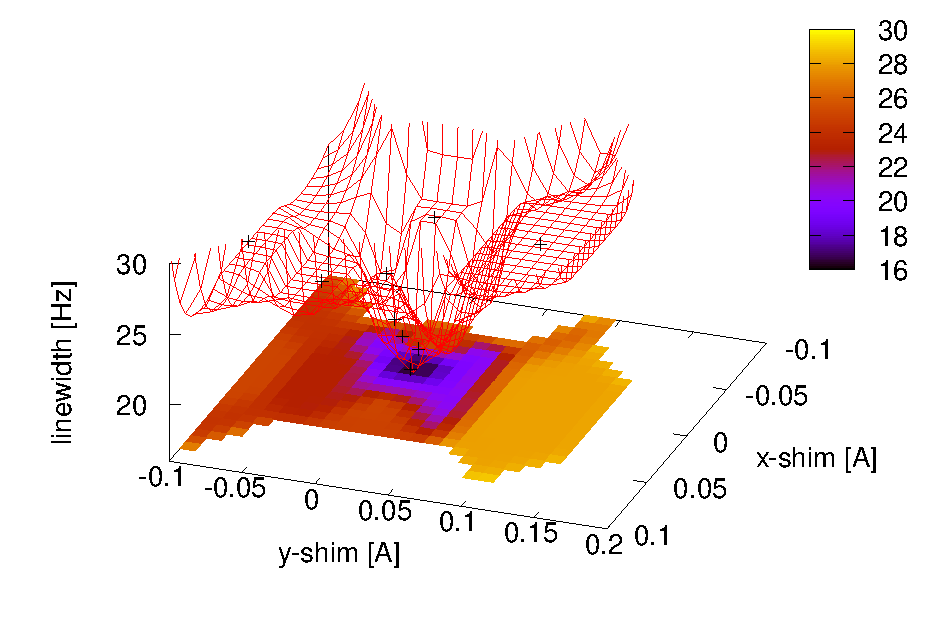
\includegraphics[width=0.9\textwidth]{/figures/experiments/lowFieldSpectrometer/shims/shimXY.eps}
                \caption{Linear shimmung in x- and y-directions. Shimming was done manually: 1H spectra of water were recorded and evaluated as to their linewidth. Later, automatic shimming was implemented (see section \ref{chap:MaterialsAndMethods:lowFieldSpectrometer:shims})}
            \end{figure}
    \subsection{Sabre shuttling system}
        The system designed to transfer a sample between fields works as intended. Fluid losses are
        small and acceptable with about \todo{how much} lost within \todo{nn} shuttling cycles. The
        bubbling system works well and provides pH2 to the solution in large amounts. The pressure
        stability of the vessels has been tested to withstands up to $\SI{50}{\bar}$. Simulations results indicate a factor of safety of $\gamma = 4$ \ref{fig:results:bubblingReactorPressure}.
        \begin{figure}
            \label{fig:results:bubblingReactorPressure}
            \centering
            \includegraphics[width = 0.9\textwidth]{/figures/simulations/15NSabre/bubblingReactorPressure.eps}
            \caption{Wall stress of the low field reactor for bubbling pH2 at \SI{200}{\bar}. As expected, the most vulnerable part is the long side of the cylinder, but wall thickness of \SI{3}{\milli\meter} suffices for a factor of safety of 4 if the setup is operated at \SI{50}{\bar} max.}
        \end{figure}
        
        Chemical resistance is good though resistance to pure pyridine is not given. While there was never
        any problem with the $\SI{}{\milli\Molar}$ pyridine concentrations used in the experiments, a
        neat pyridine batch showed to dissolve the PSU casing.
        \subsubsection{Shuttling reproducibility}
        To ensure that the sample is removed completely from the high field side, spectra in both 'states' of the system were recorded (\ref{fig:results:15N:shuttlingRemoval)}. Integration over both spectra yielded a upper limit of sample remaining inside the high field chamber of which corresponds to an effective polarization reduction of \SI{1}{\percent}.
        \begin{figure}
            \label{fig:results:15N:shuttlingRemoval}
            \centering
            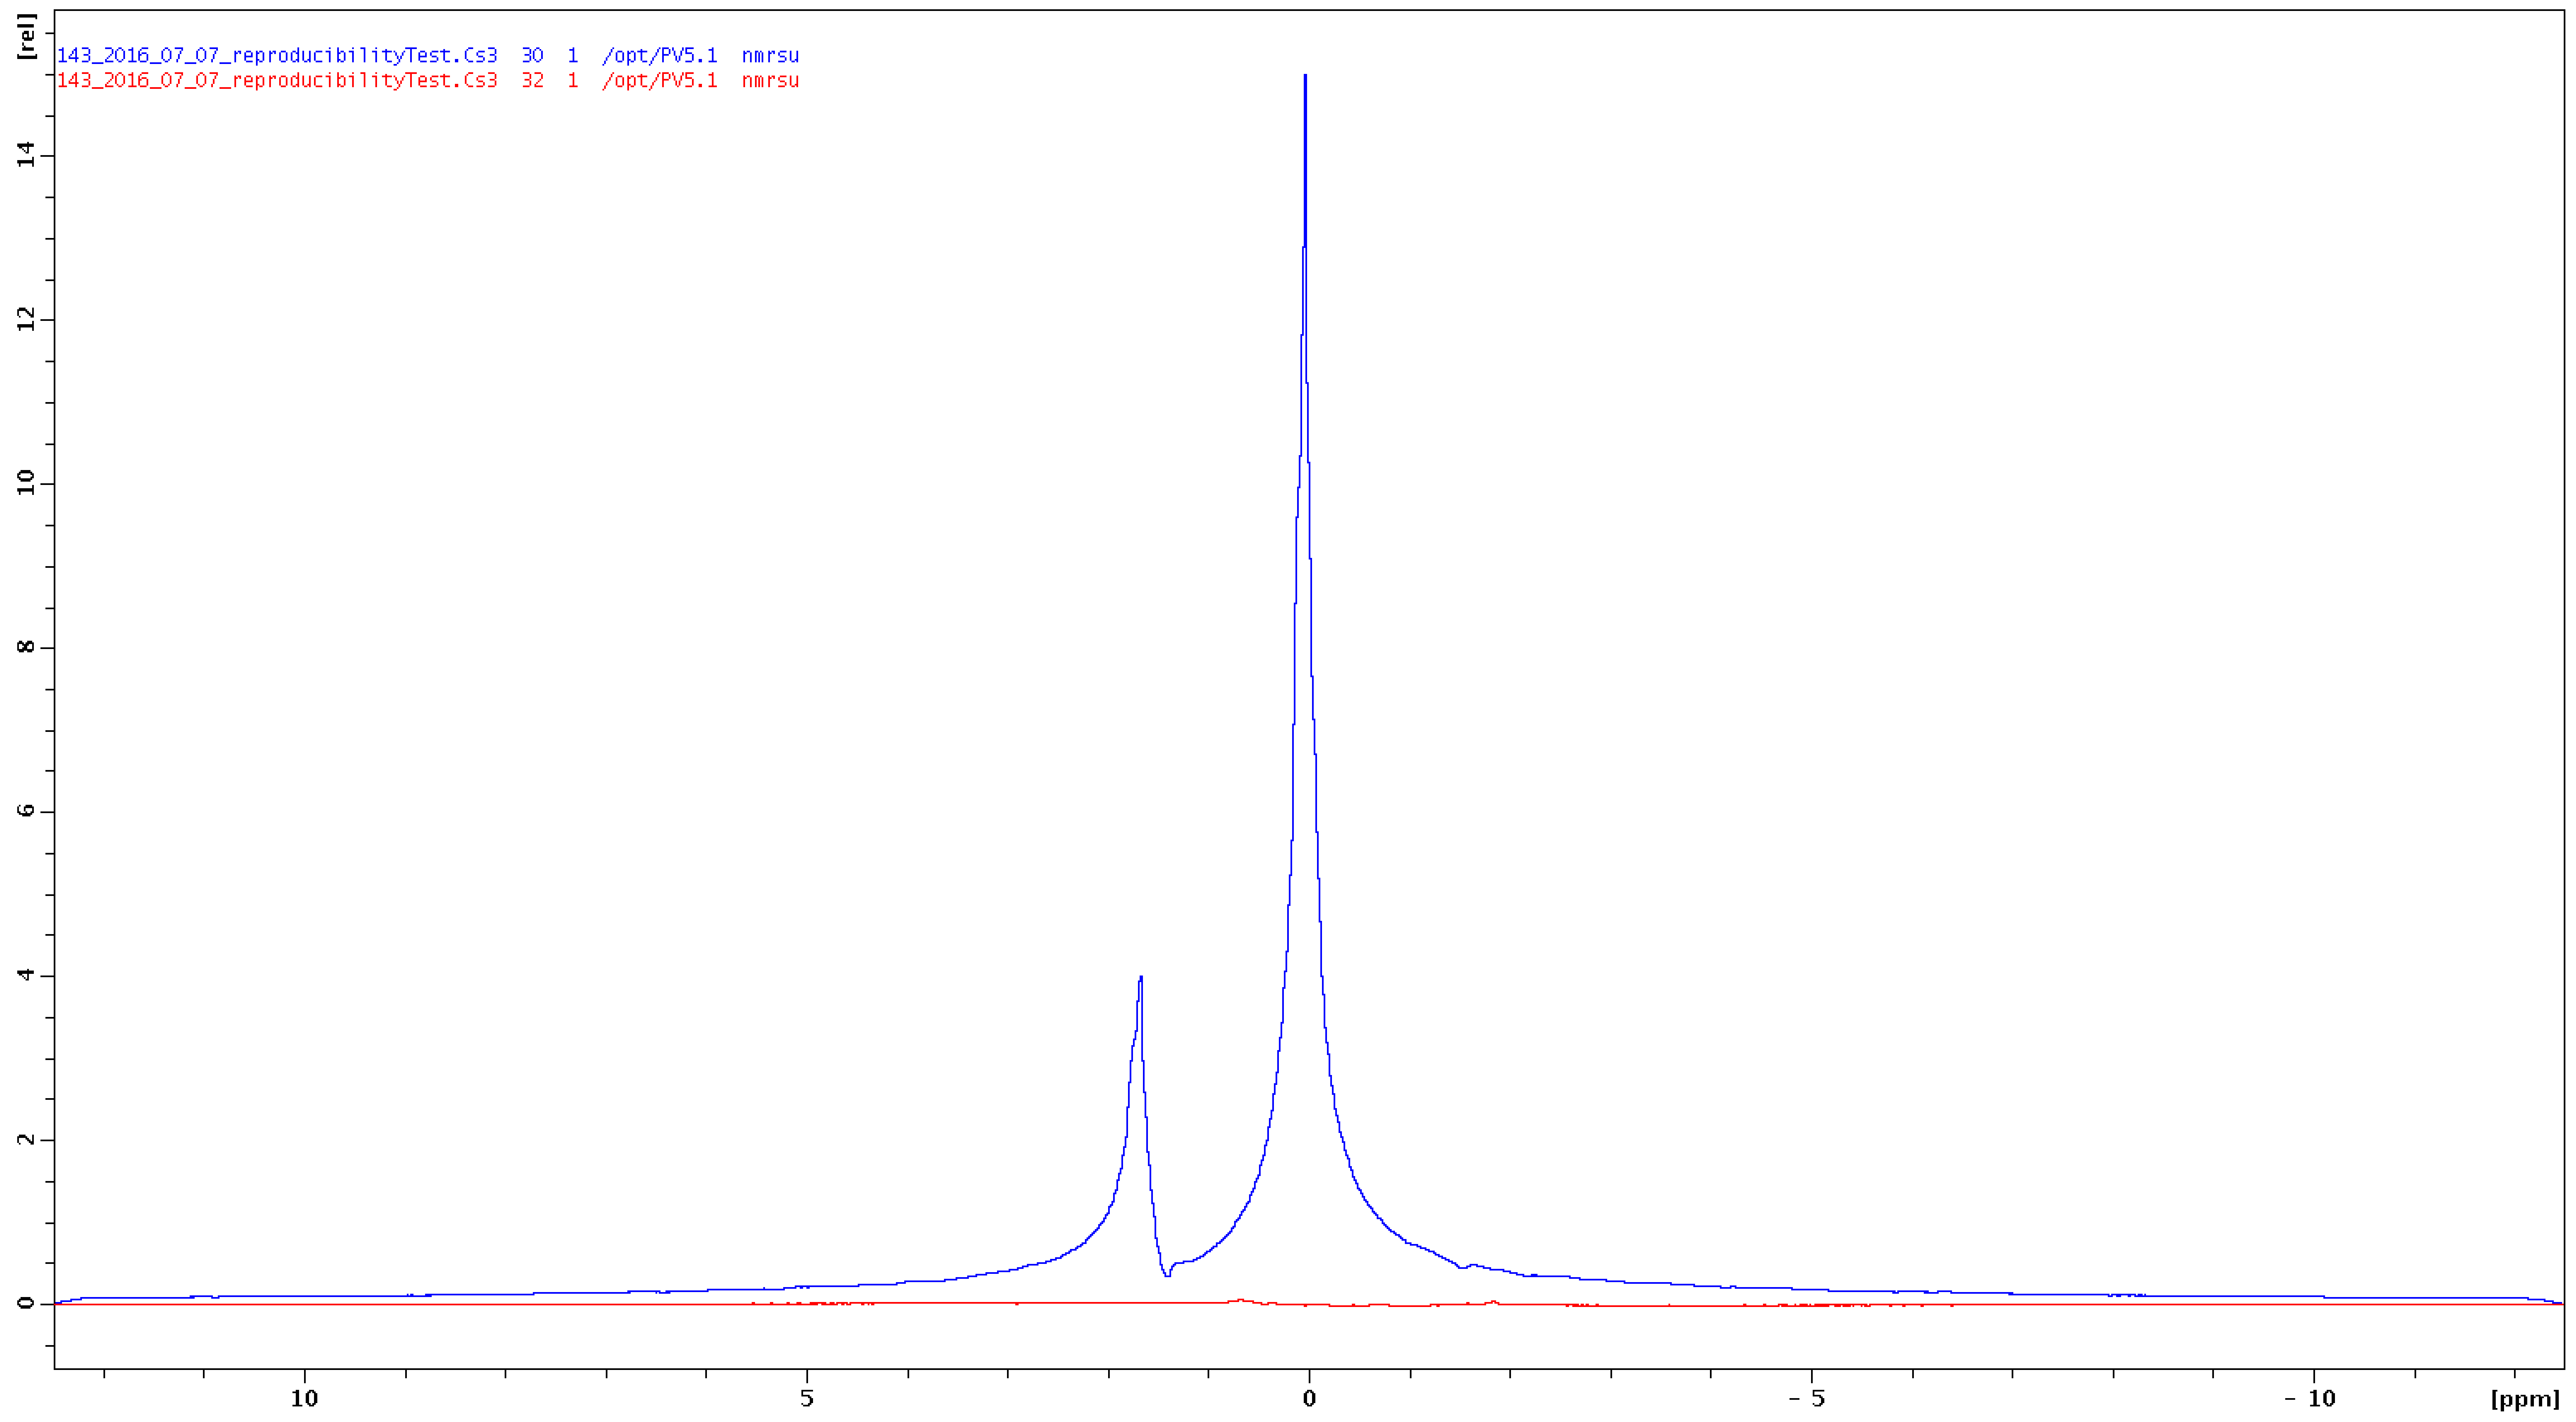
\includegraphics[width=0.9\textwidth]{/figures/experiments/15NSabre/reproducibility/spectraComparisonShuttle.eps}
            \caption{1H spectra of the high field reactor in the filled (blue) and empty (red) state. The filled state delivers a lot more signal as expected while the integration over the empty state spectrum shows a signal reduction of 1000.}
        \end{figure}
        To test the reproducibility of the shuttling system, a hyperpolarized 1H pyridine sample was shuttled back and forth multiple times. The results of the measurement are shown in figure \ref{fig:results:15N:shuttlingReproducibility}. 
        \begin{figure}
            \label{fig:results:15N:shuttlingReproducibility}
            \centering
            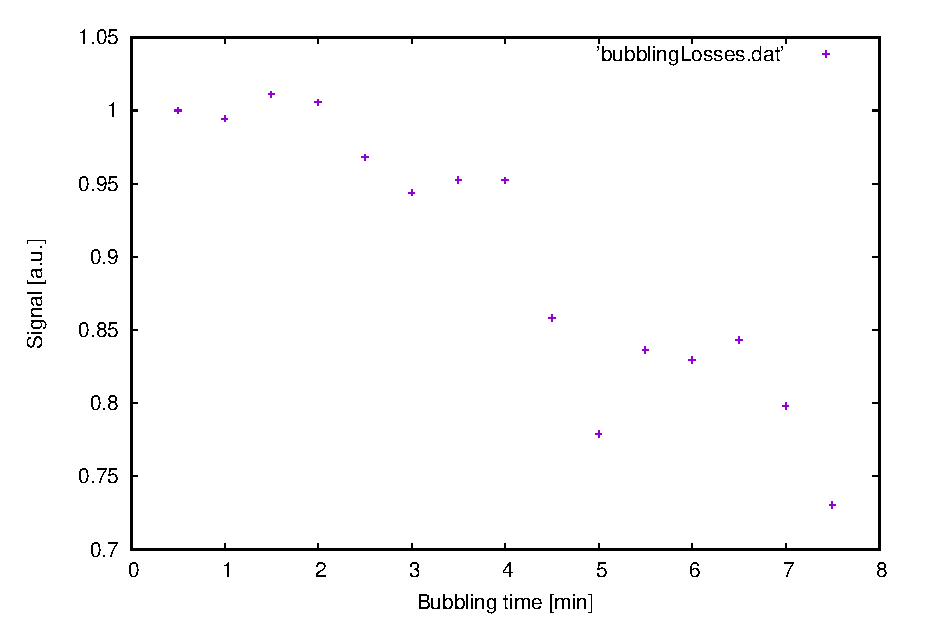
\includegraphics[width=0.9\textwidth]{/figures/experiments/15NSabre/reproducibility/bubblingLosses.eps}
            \caption{Signal intensity during multiple minutes of hydrogen bubbling using a hyperpolarized 1H-pyridine sample. Note that the signal drops to about \SI{70}{\percent} of its initial value after 8 minutes of continuous hydrogen supply. The initial rise of signal during the first two minutes indicates a temperature effect unaccounted for.}
        \end{figure}
    \subsection{Fluxgate readout electronics}
        The readout electronics were designed to feature a wide range of amplifications for all
        three spatial dimensions. A 24 V DC power supply was fitted with a DC-DC-converter to
        provide the $\pm\SI{15}{\volt}$ to power the Fluxgate. Additionally the PCB board was fitted
        with the electronic parts (see \ref{sec:methodsFluxgate}). For testing purposes, a simple program
        using serial in and output to toggle the analog switches was written. All switches were
        successfully tested to work, though three had to be replaced at some point for malfunction.
        Apparently this was due to damage during assembly as the board is now working as expected.
    \subsection{Fluxgate calibration}
    The three spatial channels of the fluxgate sensor needed to be calibrated as to their intrinsic offsets as described in \ref{materialsMethods}. Data for X- and Y-channels are shown in figure \ref{fig:results:fluxgate:xysinus}
        \begin{figure}[h]
            \label{fig:results:fluxgate:ysinus}
            \centering
            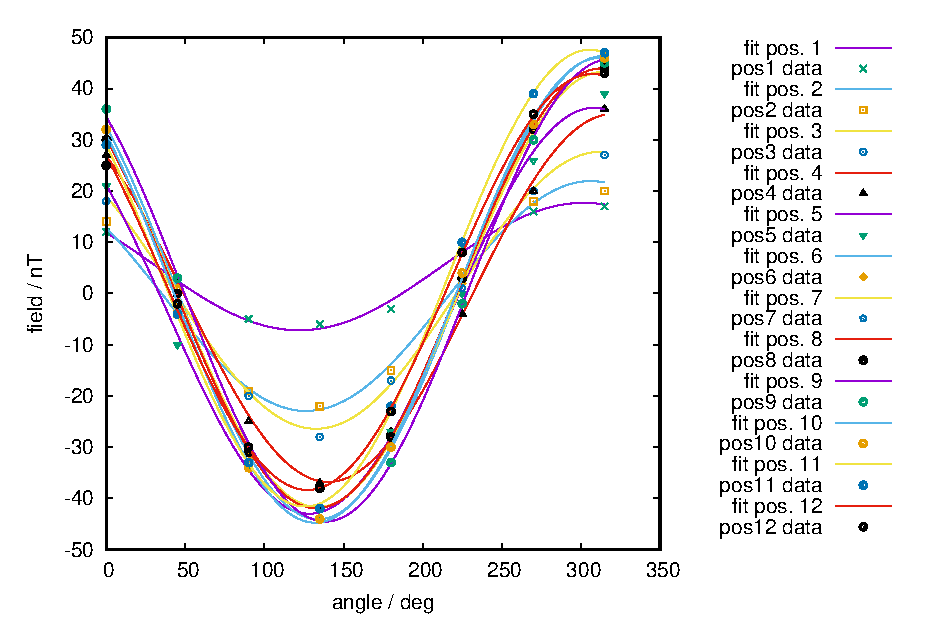
\includegraphics{/home/philipp/Documents/thesis/figures/experiments/fluxgate/xField.eps}
            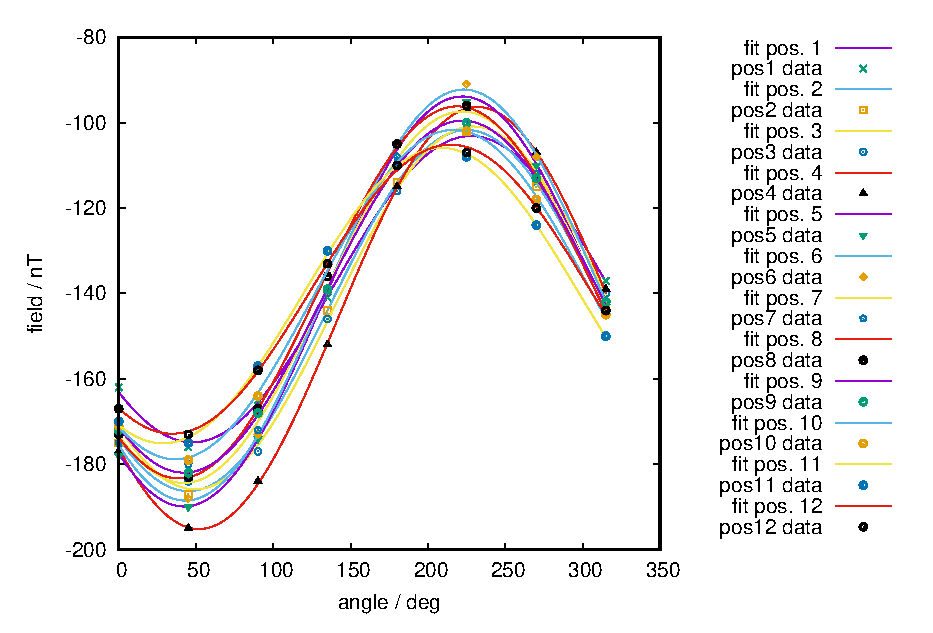
\includegraphics{/home/philipp/Documents/thesis/figures/experiments/fluxgate/yField.eps}
            \caption{Calibration data of X- and Y-channel. Each dataset in the key corresponds to a full rotation at one position in the MuMetal shield. The solid lines correspond to a sine fit to each dataset with phase, amplitude and offset as fitting parameters. Error bars are not displayed for better visibility.}
        \end{figure}
        The fit parameters shown in table \ref{table:results:calibrationFitParams} allow for calibration of X- and Y- channel by calculating the average offset for all Positions.
        \begin{table}
            \centering
            \label{table:results:calibrationFitParams}
            \begin{tabular}{r|cccccccccccc}
                \label{table:results:calibrationFitParams}
                position & 1& 2 & 3 & 4 & 5 & 6\\
                \hline
                amplitude & 22.4 & 27.0 & 35.9 & 39.6 & 45.2 & 42.5\\ 
                offset \\
                phase \\
                \hline
                position & 7 & 8 & 9 & 10 & 11 \\
                \hline
                amplitude & 42.9 & 45.1 & 45.4 & 44.6 & 40.6\\
                offset \\
                phase
            \end{tabular}
        \end{table}
        \begin{figure}[h]
            \label{fig:results:fluxgate:zcal}
            \centering
            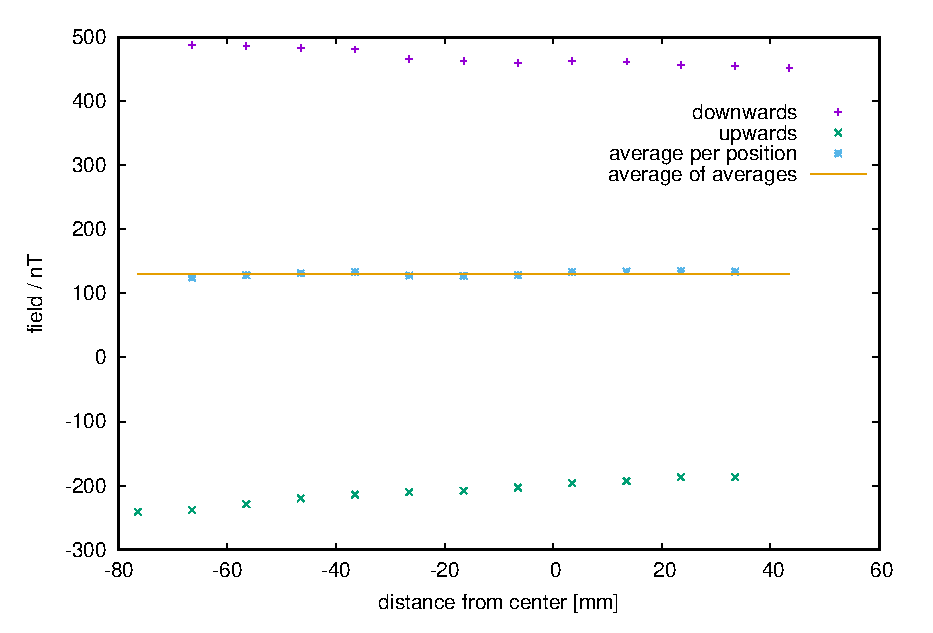
\includegraphics{/home/philipp/Documents/thesis/figures/experiments/fluxgate/zField.eps}
            \caption{Calibration of the Z-channel. Due to spatial limitations, no full rotation in z direction was possible. The two datasets represent one measurement in "upwards" ond one in "downwards" direction. The solid line represents the average of the positional averages of the two directions.}
        \end{figure}
        Using the data for calibration, the measurements of the X- and Y-channels can be used to plot a 2D-section of the field using the phase of the fit as the field direction and the amplitude as its magnitude. Both X- and Y-sensor are shown in figure \ref{fig:results:fluxgate:plotSpatial2d}. The absolute positions are indicated in the figure to enable comparison of the individual results in the same absolute position. The same data is also shown in a 3D plot (fig. \ref{fig:results:fluxgate:plotSpatial3d} to show the field progression inside the mu metal shield.
        \begin{figure}[t]
            \label{fig:results:fluxgate:plotSpatial2d}
            \centering
            %\includegraphics{/home/philipp/Documents/thesis/figures/experiments/fluxgate/spatial2dProjection.eps}
            \includegraphics{/figures/experiments/fluxgate/spatial2dProjection.eps}
        \end{figure}
        \begin{figure}[t]
            \label{fig:results:fluxgate:plotSpatial3d}
            \centering
            %\includegraphics{/home/philipp/Documents/thesis/figures/experiments/fluxgate/spatial2dProjection.eps}
            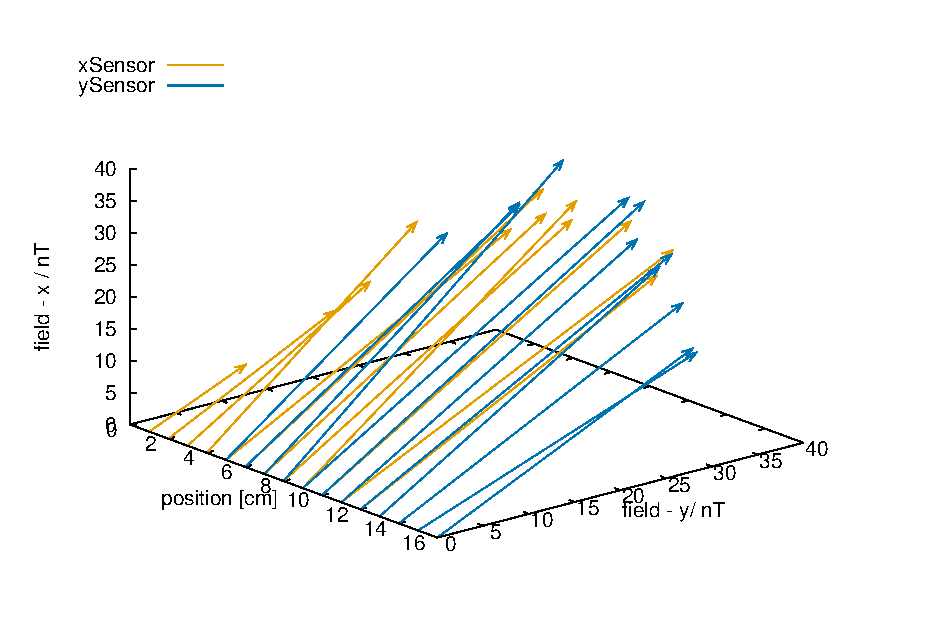
\includegraphics{/home/philipp/Documents/thesis/figures/experiments/fluxgate/spatial3d.eps}
        \end{figure}
\section{Measurements}
    \subsection{Low field NMR}
    Low field spectra were acquired using different setups. The main modification between setups concerned the $B_0$ coil. The initially used solenoid coil showed linewidths of about 0.5 - \SI{1}{\kilo\hertz}. Due to mechanical destruction of one coil and those rather wide lines, a new coil design was simulated and built \ref{simulations:DualHelmholtzArray} using Biot Savart calculations.
    \begin{figure}[h] 
        \centering
        %\includegraphics{}
    \end{figure}
    \begin{figure}[h]
        \centering
        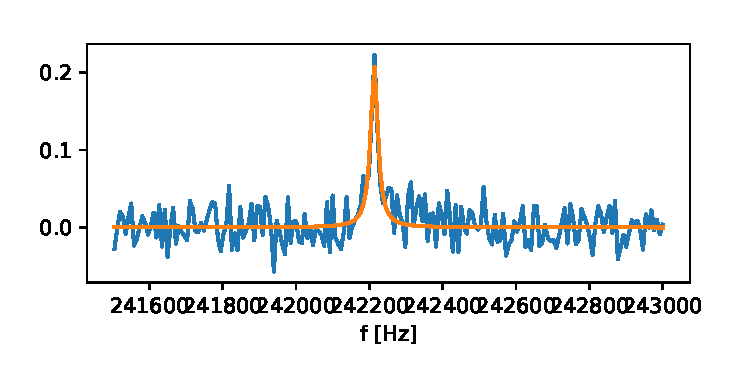
\includegraphics[width = 12cm]{/home/philipp/Documents/thesis/figures/experiments/lowFieldSpectrometer/helmholtzNarrowLine.eps}
    \end{figure}
    \subsection{Sabre in water}
    \begin{figure}[h]
        \subfloat{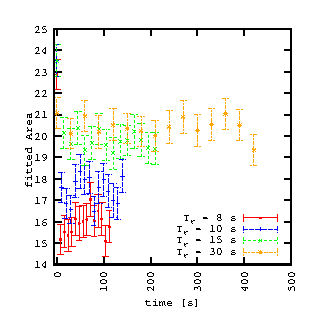
\includegraphics[width = 0.5 \textwidth]{/home/philipp/Documents/thesis/figures/experiments/lowFieldSpectrometer/inSituSabreWater/overlayAll8to30.eps}}
        \subfloat{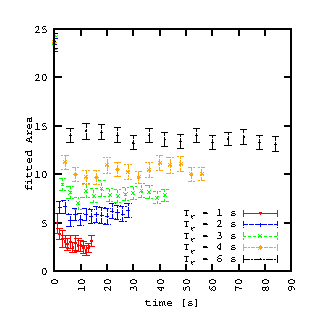
\includegraphics[width = 0.5 \textwidth]{/home/philipp/Documents/thesis/figures/experiments/lowFieldSpectrometer/inSituSabreWater/overlayAll1to6.eps}}
    \end{figure}
    \begin{figure}[h]
        \centering
        \includegraphics[width = 6 cm]{/home/philipp/Documents/thesis/figures/experiments/lowFieldSpectrometer/inSituSabreWater/exponentialFit.eps}
    \end{figure}
    \subsection{Sabre in cell solution and blood}
    \begin{figure}[h]
        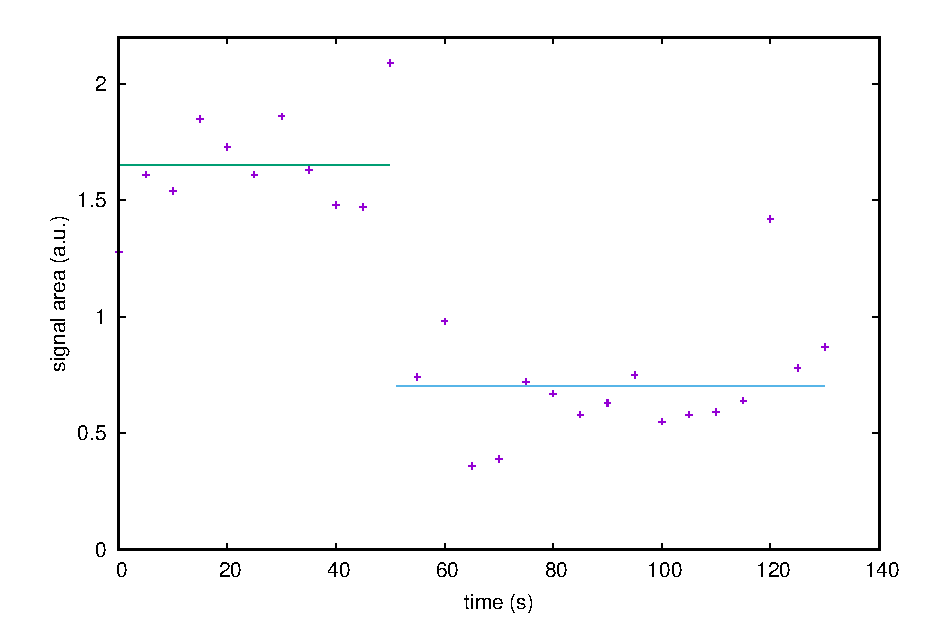
\includegraphics[width=0.9\textwidth]{/home/philipp/Documents/thesis/figures/experiments/lowFieldSpectrometer/inSituSabreWater/cellCultureInjection.eps}
        \caption{Time course of the signal intensity (peak height) when adding human blood to the continuously hyperpolarized solution. Note the string signal drop after addition of \SI{0.5}{\milli\litre} of blood to the solution. The straight and dashed lines indicate the average before and after blood addition.}
        \label{chap:MaterialsAndMethods:bloodInjection}
    \end{figure}
    \begin{figure}[h]
        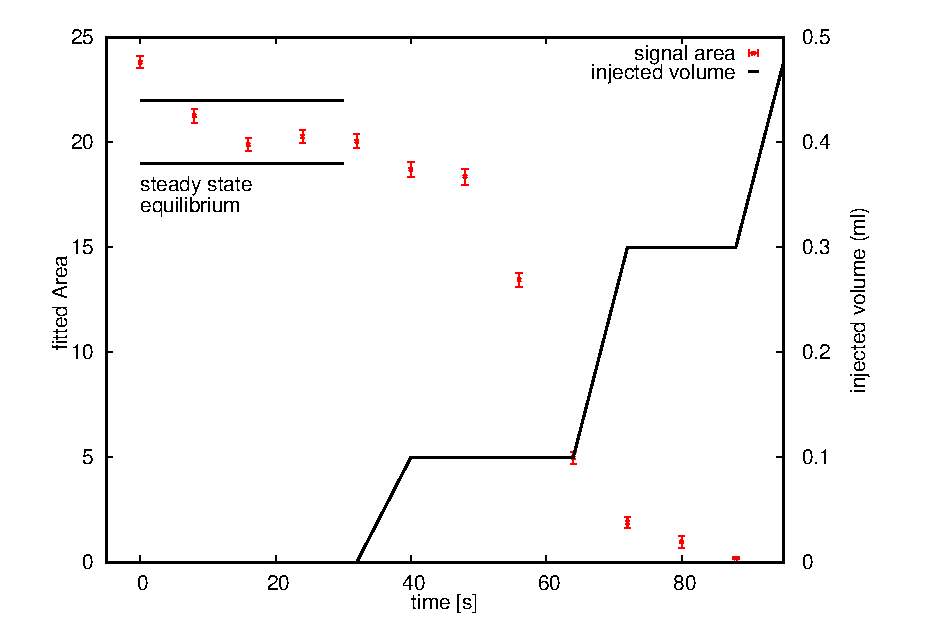
\includegraphics[width=6 in ]{/home/philipp/Documents/thesis/figures/experiments/lowFieldSpectrometer/inSituSabreWater/signalVariation.eps}
        \label{chap:MaterialsAndMethods:bloodInjection2}
        \caption{Signal drop during the injection of \SI{0.5}{\milli\liter} of blood into the solution providing hyperpolarized signal which was permanently provided with fresh pH2.}
    \end{figure}
    \subsection{15N Sabre}
        \subsubsection{15N coil}
        The coil for 15N signal reception was matched and tuned to fit the requiremenst of the system. The network analyzer showed a q-factor of \todo{n} and a width of nn. Inside the small animal NMR, similar resonance widths of nn were observed while the attenuation was \SI{1}{\deci\bel}
    \subsection{Nanotesla field measurements}
        The field inside the Mu Metal shielding was measured without anny current flowing in the B0 coil as well as with the coil turned on. 
    \subsection{High field Sabre}
\section{Simulations}
        \subsection{Static magnetic field calculations}
            Using the Biot Savart law, a Matlab program to calculate the fields of current carrying conductors was implemented. Structural elements were mostly solenoids, but also saddle and helmholtz coils were considered.
            \subsubsection{solenoid coil}
                The coil used in the low field NMR system was calculated and the length of the compensation windings was optimized for field homogeniety. To do so, the field was calculated inside a $3 x 3 x 3 cm^3$ volume centered inside the coil and plotted as histograms binning fields. An algorithm analyzing over which field 80\% of the fields sampled spread was used as a marker
            \begin{figure}[b]
                \centering
                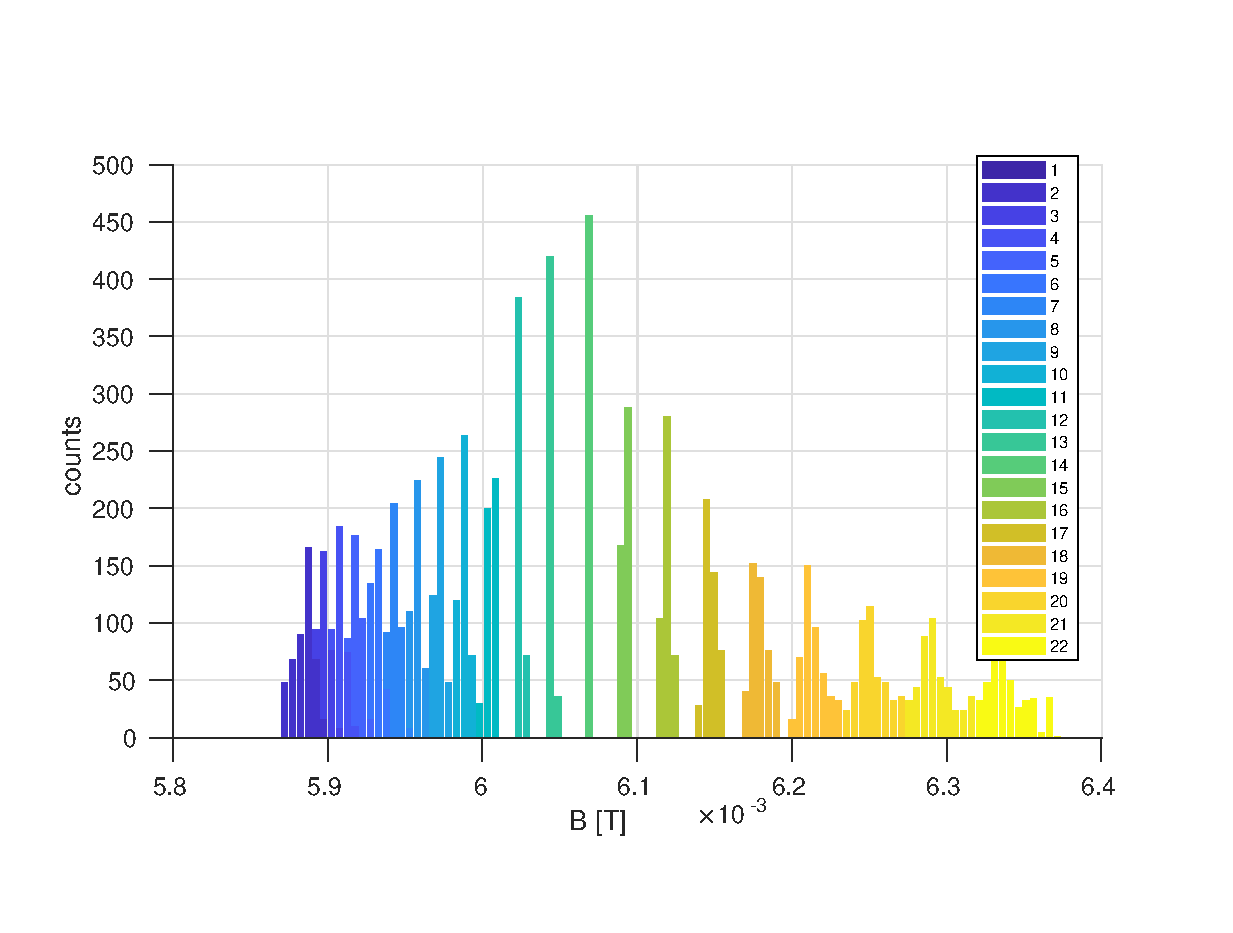
\includegraphics[width=\textwidth]{/home/philipp/Documents/thesis/figures/simulations/B0/solenoidCoil/compensationWinds.eps}
                \caption{Histograms of the magnetic field strength. From left to right, number of compensation windings rise. This leads to a field increase and change in homogeniety.}
            \end{figure}
        \subsubsection{Helmholtz Array}
        The previously used program was also used to simulate the field of the helmholtz array used in later experients. The simulations were used to optimize the parameters for the setup before manufacture. The simulation results concerning the positions of the coils are shown in figure \ref{}. The optimal result is marked, and the field homogeniety is plotted for this result (figure \ref{}). Comparing the field map to figure \ref{} shows a factor \todo{nn} improvement.
        \begin{figure}
            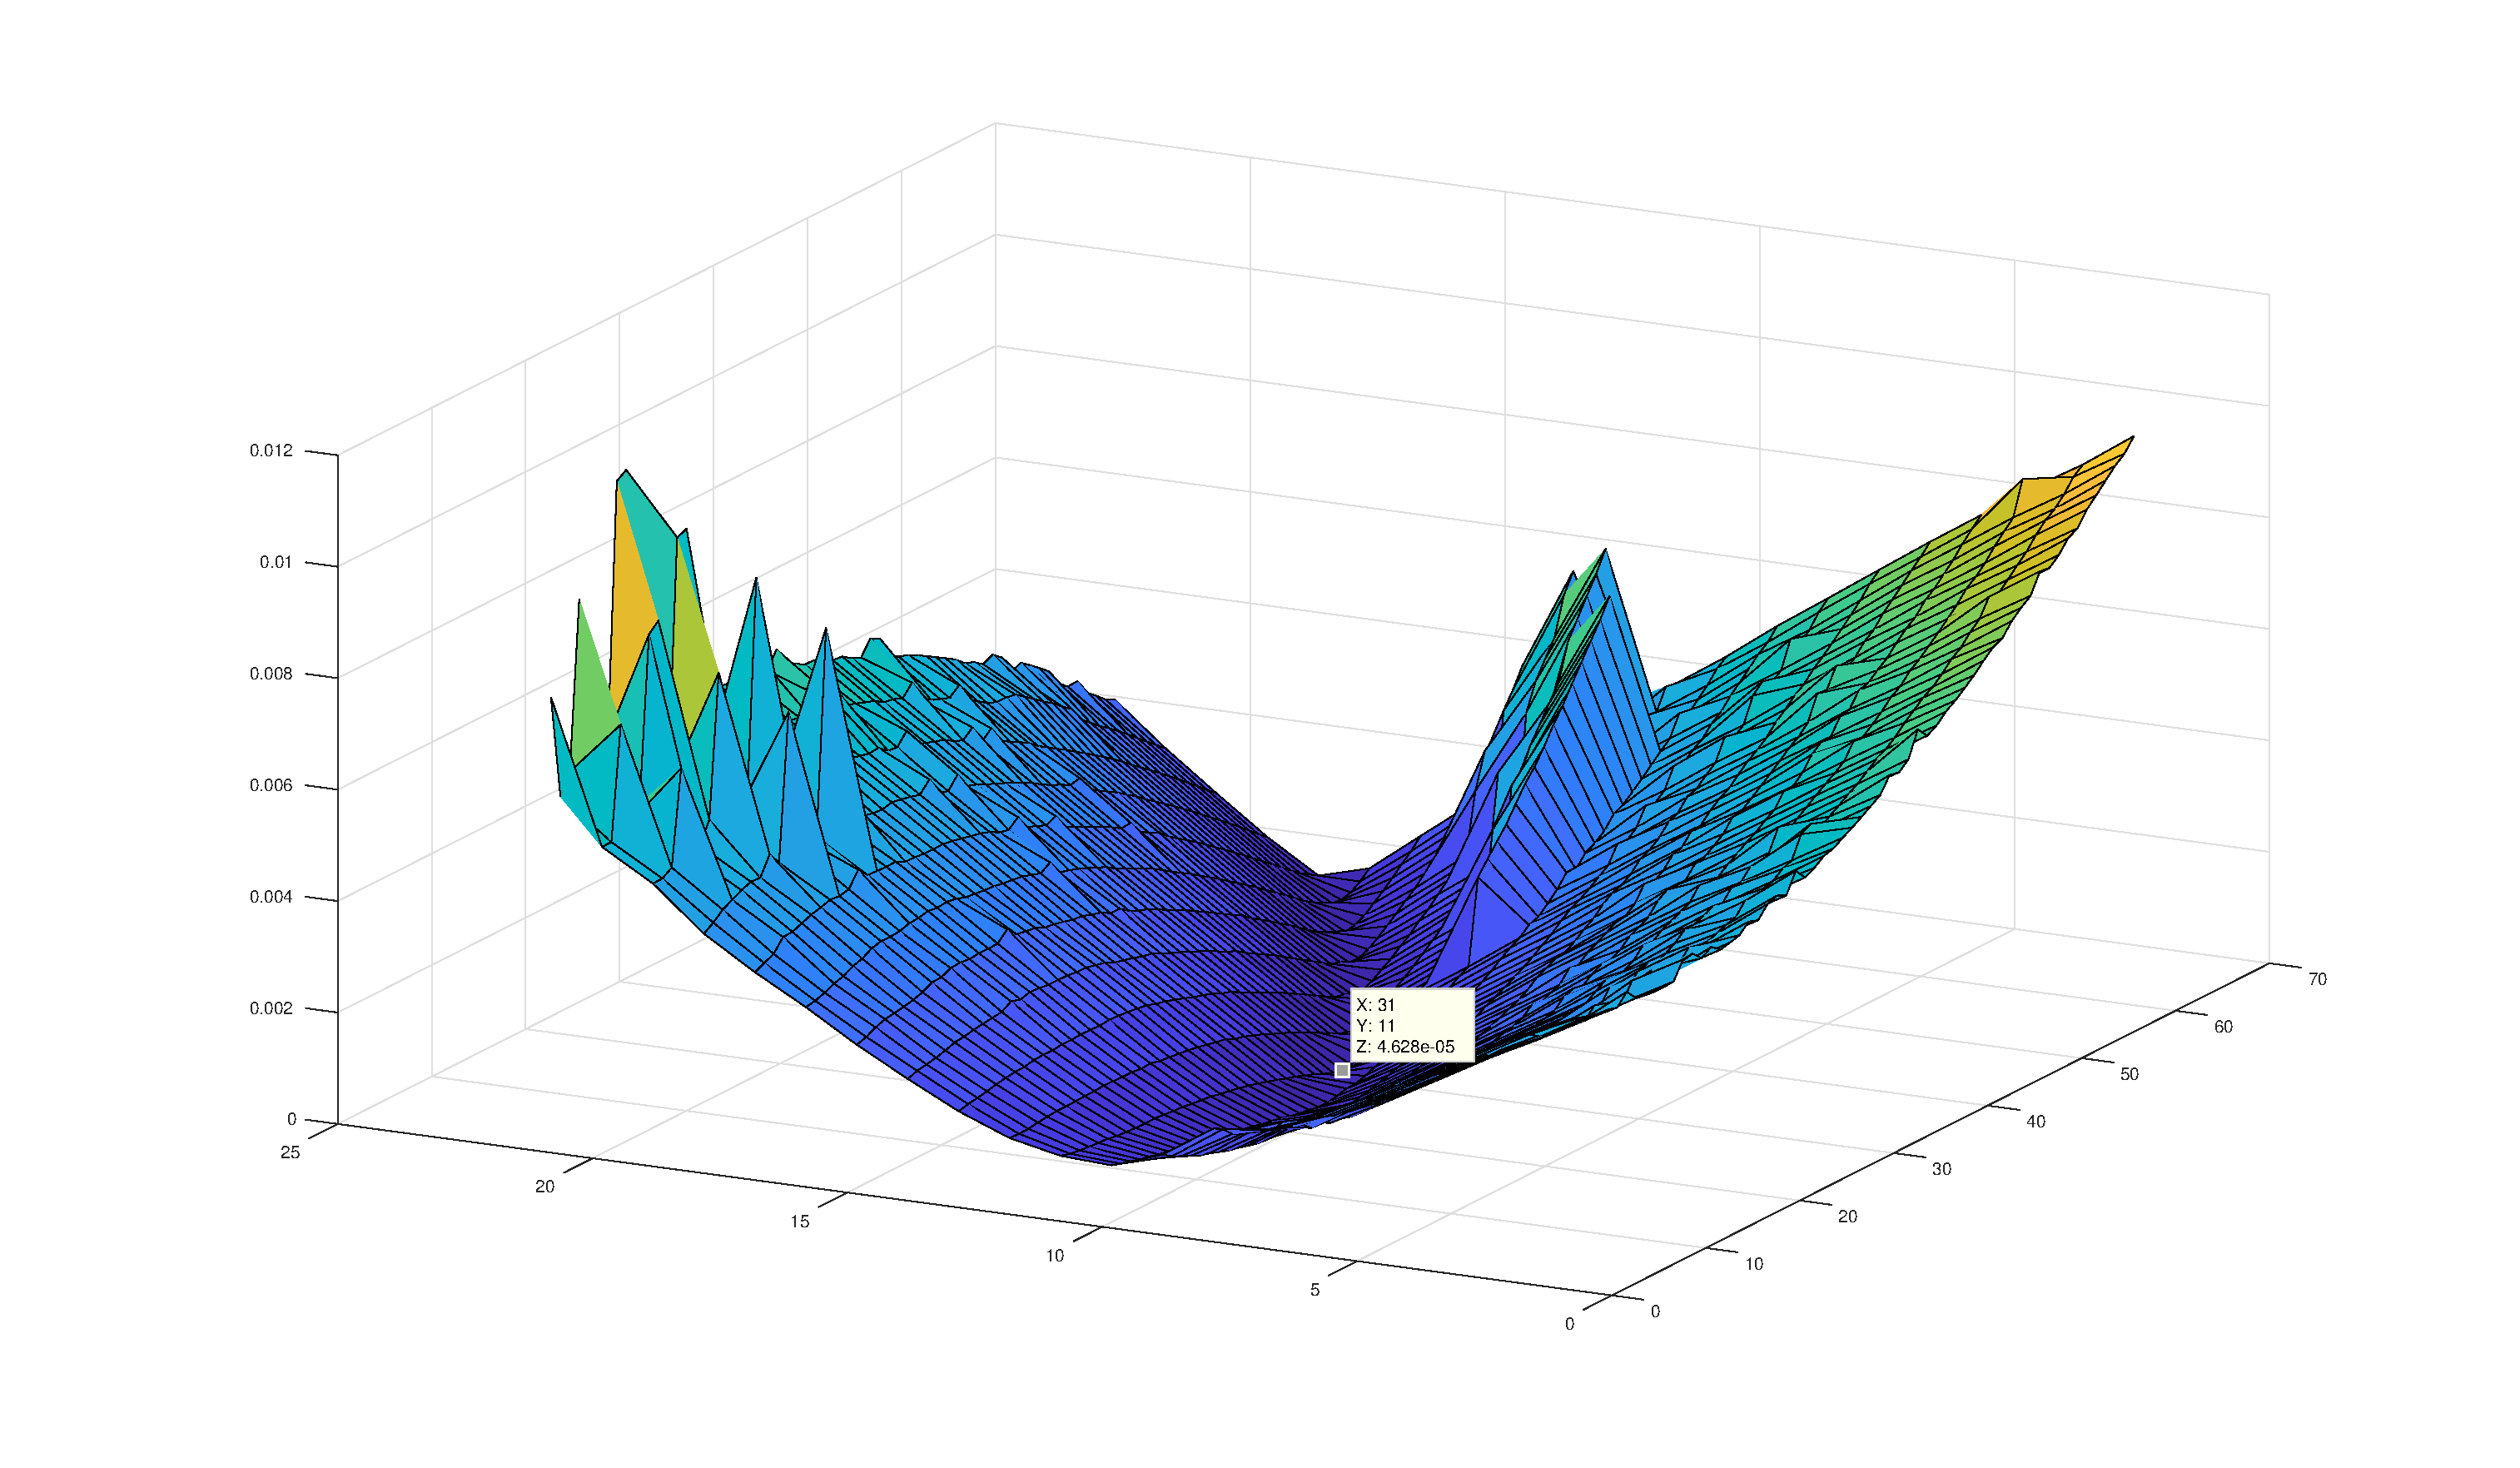
\includegraphics[width = 0.9\textwidth]{/figures/simulations/B0/helmholtzCoil/fieldSpread.eps}
        \end{figure}
%\input{figures/experiments/figExample}

    % !TEX root = ../thesis_main.tex
\chapter{Discussion and Conclusion}\label{chap:conclusion}
    \section{$B_0$ field generation}
        Multiple coil designs of the static field generating coils have been considered, simulated, built and tested in the course of this work. The previously used solenoid design with different lengths of compensation windings (section \ref{sec:results:sim:B0}) showed rather broad lines in both simulations and measurements. Main reason are the discrete number of compensation windings that do not allow for fine enough tuning of the coil. This could be improved by putting the compensation windings on sliders that can move in z-Direction. additionally in the design used, mechanical errors in the build worsened the problematic. Due to the high number of windings guided only by the previously wound wire, shifts building along the coil's z axis are inevitable. In addition, layering the wire leads to slippage into the gouge created by the previous layer. This problem may be solved by using a thin, but stiff layer of material to separate the wire layers from each other. All of the mentioed solutions are inconvenient when considering the dimensions of the coil. 
        The heating of the solenoid coil led to an additional problem: Field shifts, probably due to the thermal expansion of the copper heating by $\Delta T = \SI{40}{\kelvin}$ for the \SI{35}{\centi\meter} long coil leads to an expansion of 
        \begin{equation}
            \Delta x \approx \alpha \mathrm{L}\Delta\mathrm{T}= \SI{16.5e-6}{\per\kelvin}\cdot \SI{40}{\kelvin} \cdot \SI{0.35}{\meter} = \SI{0.2}{\milli\meter}
        \end{equation}
        This change leads to a clearly visible frequency shift that can be problematic for measurement reproducibility (compare also to simulations of sub-milimeter positioning errors, figure \ref{fig:results:fieldSpread})
        To avoid field shifts during measurements, the setup should therefore be in thermal equilibrium. This is especially relevant when switching fields during measurements using the programmable power supply.

        The dual helmholtz array design deals with the above mentioned problems. The single coils are wound onto a milled holder making moving in z direction possible and convenient. due to the shorter extension of the coils in z direction, the errors introduced in the winding process are smaller and using PVC foil to separate the axial layers kept the layers neatly wound.
        In addition, the design allows for axial access to the sample which can make experiments a lot more convenient. The disadvantage of the design are the higher currents due to the lower winding count that make need for higher current power supplies.
    \section{$B_1$ coils}
        The $B_1$ coils show expected behaviour. While single channel coils are well suited for low field experiments, dual channel coils often show low performance and sensitivity on at least one of the two channels and a two coil setup can often be more reasonable. The determined Q-factors were in the range previously mentioned in literature. 
    \section{Shims}
        Shims do work as intended. For future builds, higher order shims should be considered as the field distribution of the solenoid coils was - considering both simulations and linewidths - seemed more quadratic. Thus, linear shims did improve liewidths slightly but were not able to get beyond linewidths of \SI{50}{\hertz}. Considering the low fields, this is rather large with ~200 ppm.
    \section{Imaging at earth magnetic field}
        While the signal of hyperpolarized solution was high compared to the water sample, it has to be considered that the prepolarization magnetic field was only \SI{5}{\milli\tesla} and thus about three orders of magnitude below usual commercially available MRI. At higher magnetic fields for readout, hyperpolarized signal would remain fairly constand (neglecting changed relaxation effects). Thermal signal of the pure water wuould increase linearly with the field though and thus, a high field imager is to be preferred over a low field hyperpolarized signal considering singnal only. If, though, a metabolic process could be monitored with the hyperpolarizzed nicotinamide, the setup would allow for doing this with the low concentrations provided and fairly low signal background. Furthermore, the signal increase can be used to build cheap low field imagers in specific fields such as transportable machines or low cost machines e.g. for developing countries. Here, the rather comlicated procedure has to be considered though and a system that is more automated would be necessary.
    \section{Sabre Shuttling System}
        The system was designed to perform measurements in a well reproducable setting. As all shuttling and even scanner control are automated, volumes and timings are very well reproduced within consecutive scans.
        \subsection{Temperature control}
        \label{cd:sabreShuttling:tempControl}
            Temperature is the one factor that is both not controlled and also very difficult to contorl in this setting. Wall thickness has to be in a range that withstands the pressures used in the setup and thus makes all indirect heating through the walls difficult, especially since the fluid voulme is small compared to the PSU volume surrounding it. Temperature measurement would be easily possible through optical, contactless sensors, but temperature control is not solved. Optimal temperatures for the IR-IMes/Methanol/15N-pyridine mixture were shown to be at around \SI{14}{\celsius}. As these temperatures are below laboratory AC temperatures of \SI{18}{\celsius} and the parahydrogen flow decreases the sample's temperature, the optimal temperature was reached (experiments show temperature decreases towards \SI{0}{\celsius} under constant flow), but may well be undercut. As temperature is not controlled or regulated in the current setup, a sleeve for a cooling or heating liquid may be considered in future designs. \todo{fig temp sleeve}.
        \subsection{Shuttling speeds}
            The duration of the shuttling procedure was short enough to keep hyperpolarization at levels sufficient for analysislevels. For future setups, a additional field that can be switched on before shuttling starts should be considered as T1 relaxation at \SI{}{\nano\tesla} fields is a lot faster (~ \SI{1}{second}). Fields of \SI{1}{\micro\tesla} suffice to increase relaxation times (pyridine in methanol) to \todo{times} \SI{10}{\second}. 
        \subsection{Shuttling reproducibility}
            As shown in section \ref{results:15N:shuttlingReproducibility}, the relative error on the shuttling process is low. It has to be considered thoug that a completely dry system will reduce the amount of substance arriving on the high field side by a non neglectable amount by humidification of the surfaces. That is why, depending on the previous state of the system, a drop in signal could be observed during the first or first two shuttling procedures. After that, the only source of loss is the evaporation of liquid during bubbling. High flows generate high polarization and signal yield up to a certian point, but also cause large losses in fluid volume over short periods of time. Therefore, for parameter optimization, usually  a lower flow rate was chosen to make consecutive scans more comparable. The scaling with flow should be independent of the other parameters and can therefore be adapted accordingly.
        \subsection{Pressure dependence}
            Polarization shows a linear dependence on pressure in the measured range. This indicates that higher pressures would still increase the signal as a plateau is to be expected where a higher pH2 concentration in solution does not increase reaction rates at the catalyst any more because it already is steadily available. Increasing pressures further in future setups is certainly possible considering the still rather thin walls of the PSU reactors. One limitation that occurs are certainly the screwed ferrule connections of the capillary and PTFE tubing which, under high pressures can slip uot of its fit. It can be replaced by more sophisticated flanged ferrule connections which require special tools that are commercially available though. Larger inner diameter tubing also starts to reach its pressure limitations above \SI{50}{\bar}, but can easily be replaced by tubings with smaller inner diameter. Reduced flow through these tubings will, on the one hand, be compensated by the higher pressure differences themselves, on the other hand, the only fluid pathway is already covered by a small diameter capillary resisting pressures up to \SI{200}{\bar} according to its data sheet.
        \subsection{Field dependence}
            The dependence on the magnetic field shows a pattern of two peaks around a minumum with signal going towards 0 in the outskirts, i.e. towards high fields. This makes sense as simulations suggest fields around \SI{300}{\nano\tesla} delivering the energy splitting range in which level anti crossings are fully developed. The overall field depends on the residual magnetization of the mu metal shielding and is measured indepently. That makes direct comparisons difficult as the shield needs to be opened to change from measurement head (fluxgate) to the polarization system. During that exchange magnetization of the shield can change by mecahnical stress such as hits to the shields or lids or by externel magentic fields reaching into the inner shields and leaving residue magnetization even after opening.The asymmetry of the distribution is due to residual magnetic field of the shield. It generates both a shift of the 'mirror axis' and an overall deformation of the distribution depending on the field homogeniety.

        \subsection{Concentration dependence}
            The concentration plays an important role in the Sabre complex formation, the formation of different intermediates and also the disassembly of the complexes. Generally, a concentration that is large compared to the catalyst concentration will lead to a reduction in polarization as the pool of substrate molecules in solution is large compared to those in bound form. This can be seen from the data, as a reduction of the relative concentration of susbtrate leads to a signal increase. Catalyst concentration remains constant in the example given. This means that, although the overall amount of substance of the substrate does not change, more molecules are hyperpolarized at the same time and thus a larger magnetization is generated.
        \subsection{Polarization and magnetization}
            Polarization reached levels in the previosly reported ranges while magnetization was high considering the high concentrations of \SI{50}{\milli\molar}. Many publications seem to try and maximize polarization - in this work, magnetization, i.e. absolute signal intensity was considered more important as for any future application, this is the more relevant parameter.

    \chapter{Acknowledgments}

First and foremost, I would like to thank...
\begin{itemize}
\item{advisers}
\item{examiner}
\item{person1 for the dataset}
\item{person2 for the great suggestion}
\item{proofreaders}
\end{itemize}

    % bibliography is not in the table of contents per default, add it manually
    % enable the \renewcommand for german header
    % \renewcommand{\bibname}{Literaturverzeichnis}
    \addcontentsline{toc}{chapter}{Bibliography}
    
    \bibliographystyle{ieeetr}
    \bibliography{bib/topic1}
    \newpage
    \thispagestyle{empty}
    \mbox{}
    

\end{document}
